\documentclass{article}


% if you need to pass options to natbib, use, e.g.:
%     \PassOptionsToPackage{numbers, compress}{natbib}
% before loading neurips_2024


% ready for submission
\usepackage{neurips_2024}


% to compile a preprint version, e.g., for submission to arXiv, add add the
% [preprint] option:
%     \usepackage[preprint]{neurips_2024}


% to compile a camera-ready version, add the [final] option, e.g.:
%     \usepackage[final]{neurips_2024}


% to avoid loading the natbib package, add option nonatbib:
%    \usepackage[nonatbib]{neurips_2024}


\usepackage[utf8]{inputenc} % allow utf-8 input
\usepackage[T1]{fontenc}    % use 8-bit T1 fonts
\usepackage{hyperref}       % hyperlinks
\usepackage{url}            % simple URL typesetting
\usepackage{booktabs}       % professional-quality tables
\usepackage{amsfonts}       % blackboard math symbols
\usepackage{nicefrac}       % compact symbols for 1/2, etc.
\usepackage{microtype}      % microtypography
\usepackage{xcolor}         % colors

\usepackage{color}
% \usepackage[usenames,dvipsnames]{xcolor}         % colors
\definecolor{darkblue}{rgb}{0,0,1}
\usepackage[utf8]{inputenc} % allow utf-8 input
\usepackage[T1]{fontenc}    % use 8-bit T1 fonts
% \usepackage[colorlinks=true,
%             urlcolor=purple,
%             linkcolor=red,
%             citecolor=blue]{hyperref}       % hyperlinks
% \usepackage{hyperref}
% \usepackage{url}            % simple URL typesetting
\usepackage{graphicx}
\usepackage{subcaption}
\usepackage{amsmath}
\usepackage{amssymb}
\usepackage{amsthm}

\usepackage{wrapfig}
\usepackage{algorithm}
\usepackage{algpseudocode}
\def\Real{\mathop{\mathbb{R}}\nolimits}
\def\dom{\mathop{\bf dom}\nolimits}
\def\argmin{\mathop{\rm argmin}\nolimits}
\def\argmax{\mathop{\rm argmax}\nolimits}
\newcommand{\svskip}{\vspace{1.75mm}}
\newcommand{\ba}{\boldsymbol{a}}
\newcommand{\bb}{\boldsymbol{b}}
\newcommand{\bc}{\boldsymbol{c}}
\newcommand{\bd}{\boldsymbol{d}}
\newcommand{\be}{\boldsymbol{e}}
\newcommand{\bff}{\boldsymbol{f}}
\newcommand{\bg}{\boldsymbol{g}}
\newcommand{\bh}{\boldsymbol{h}}
\newcommand{\bi}{\boldsymbol{i}}
\newcommand{\bj}{\boldsymbol{j}}
\newcommand{\bk}{\boldsymbol{k}}
\newcommand{\bl}{\boldsymbol{l}}
% \newcommand{\bm}{\boldsymbol{m}}
\newcommand{\bn}{\boldsymbol{n}}
\newcommand{\bo}{\boldsymbol{o}}
\newcommand{\bp}{\boldsymbol{p}}
\newcommand{\bq}{\boldsymbol{q}}
\newcommand{\br}{\boldsymbol{r}}
\newcommand{\bs}{\boldsymbol{s}}
\newcommand{\bt}{\boldsymbol{t}}
\newcommand{\bu}{\boldsymbol{u}}
\newcommand{\bv}{\boldsymbol{v}}
\newcommand{\bw}{\boldsymbol{w}}
\newcommand{\bx}{\boldsymbol{x}}
\newcommand{\by}{\boldsymbol{y}}
\newcommand{\bz}{\boldsymbol{z}}
\newcommand{\bmu}{\boldsymbol{\mu}}
\newcommand{\bA}{\boldsymbol{A}}
\newcommand{\bB}{\boldsymbol{B}}
\newcommand{\bC}{\boldsymbol{C}}
\newcommand{\bD}{\boldsymbol{D}}
\newcommand{\bE}{\boldsymbol{E}}
\newcommand{\bF}{\boldsymbol{F}}
\newcommand{\bG}{\boldsymbol{G}}
\newcommand{\bH}{\boldsymbol{H}}
\newcommand{\bI}{\boldsymbol{I}}
\newcommand{\bJ}{\boldsymbol{J}}
\newcommand{\bK}{\boldsymbol{K}}
\newcommand{\bL}{\boldsymbol{L}}
\newcommand{\bM}{\boldsymbol{M}}
\newcommand{\bN}{\boldsymbol{N}}
\newcommand{\bO}{\boldsymbol{O}}
\newcommand{\bP}{\boldsymbol{P}}
\newcommand{\bQ}{\boldsymbol{Q}}
\newcommand{\bR}{\boldsymbol{R}}
\newcommand{\bS}{\boldsymbol{S}}
\newcommand{\bT}{\boldsymbol{T}}
\newcommand{\bU}{\boldsymbol{U}}
\newcommand{\bV}{\boldsymbol{V}}
\newcommand{\bW}{\boldsymbol{W}}
\newcommand{\bX}{\boldsymbol{X}}
\newcommand{\bY}{\boldsymbol{Y}}
\newcommand{\bZ}{\boldsymbol{Z}}
\newcommand{\balpha}{\boldsymbol{\alpha}}
%\newcommand{\bbeta}{\boldsymbol{\beta}}
\newcommand{\bbeta}{\boldsymbol{\beta}}
\newcommand{\bgamma}{\boldsymbol{\gamma}}
\newcommand{\bdelta}{\boldsymbol{\delta}}
\newcommand{\bepsilon}{\boldsymbol{\epsilon}}
\newcommand{\blambda}{\boldsymbol{\lambda}}
\newcommand{\bnu}{\boldsymbol{\nu}}
\newcommand{\bphi}{\boldsymbol{\phi}}
\newcommand{\bpi}{\boldsymbol{\pi}}
\newcommand{\bsigma}{\boldsymbol{\sigma}}
\newcommand{\btheta}{\boldsymbol{\theta}}
\newcommand{\bomega}{\boldsymbol{\omega}}
\newcommand{\bxi}{\boldsymbol{\xi}}
\newcommand{\bGamma}{\boldsymbol{\rho}}
\newcommand{\bDelta}{\boldsymbol{\Delta}}
\newcommand{\bTheta}{\boldsymbol{\Theta}}
\newcommand{\bLambda}{\boldsymbol{\Lambda}}
\newcommand{\bXi}{\boldsymbol{\Xi}}
\newcommand{\bPi}{\boldsymbol{\Pi}}
\newcommand{\bOmega}{\boldsymbol{\Omega}}
\newcommand{\bUpsilon}{\boldsymbol{\Upsilon}}
\newcommand{\bPhi}{\boldsymbol{\Phi}}
\newcommand{\bPsi}{\boldsymbol{\Psi}}
\newcommand{\bSigma}{\boldsymbol{\Sigma}}
\newcommand{\ha}{\hat{\balpha}}
\newcommand{\hb}{\hat{\bbeta}}
\newcommand{\X}{\mathcal{X}}
\newcommand{\add}[1]{{\color{red}{#1}}}
\newcommand{\M}{\mathcal{M}}
\newcommand{\I}{\mathcal{I}}
\newcommand{\E}{\mathbb{E}}
\newcommand{\F}{\mathcal{F}}
\newcommand{\J}{\mathcal{J}}
\newcommand{\cL}{\mathcal{L}}
\newcommand{\cO}{\mathcal{O}}
\newcommand{\lc}{\tau_{\balpha,k}}
%\newcommand{P}{\mathbb{P}}
\newcommand{\hth}{\widehat{\bTheta}_n}
\newcommand{\tm}{\widehat{\bTheta}_n^{(\text{MoM})}}
\usepackage{bm}
\usepackage{bbm}
\newcommand{\C}{\mathcal{C}}
% \newcommand{\bm}{\boldsymbol{#1}}
\newcommand{\sP}{\mathbbm{P}}
% \newcommand{\Pn}{\mathbbm{P}_n}

\usepackage{booktabs}
\usepackage{makecell}
\usepackage{multirow}

\newcommand{\one}{\mathbbm{1}}
\usepackage{algorithm}
\usepackage{algpseudocode}

\makeatletter
\newenvironment{breakablealgorithm}
  {% \begin{breakablealgorithm}
   \begin{center}
     \refstepcounter{algorithm}% New algorithm
     \hrule height.8pt depth0pt \kern3pt% \@fs@pre for \@fs@ruled
     \renewcommand{\caption}[2][\relax]{% Make a new \caption
       {\raggedright\textbf{\fname@algorithm~\thealgorithm} ##2\par}%
       \ifx\relax##1\relax % #1 is \relax
         \addcontentsline{loa}{algorithm}{\protect\numberline{\thealgorithm}##2}%
       \else % #1 is not \relax
         \addcontentsline{loa}{algorithm}{\protect\numberline{\thealgorithm}##1}%
       \fi
       \kern2pt\hrule\kern2pt
     }
  }{% \end{breakablealgorithm}
     \kern8pt\hrule\relax% \@fs@post for \@fs@ruled
   \end{center}
  }
\makeatother

\usepackage{comment}

\makeatletter
\renewcommand{\fnum@algorithm}{\fname@algorithm}
\makeatother

\newtheorem{thm}{Theorem}[section]
\newtheorem{lemma}{Lemma}[section]
\newtheorem{cor}{Corollary}[section]
\newtheorem{assumption}{A\hspace{-2pt}}
\newtheorem{remark}{\textbf{Remark}}
\newtheorem{eg}{Example}[section]
\newtheorem{defn}{Definition}

\usepackage{mathrsfs}

\allowdisplaybreaks


\title{Robust and Automatic Data Clustering:\\ Dirichlet Process meets Median-of-Means}


% The \author macro works with any number of authors. There are two commands
% used to separate the names and addresses of multiple authors: \And and \AND.
%
% Using \And between authors leaves it to LaTeX to determine where to break the
% lines. Using \AND forces a line break at that point. So, if LaTeX puts 3 of 4
% authors names on the first line, and the last on the second line, try using
% \AND instead of \And before the third author name.


\author{%
  David S.~Hippocampus\thanks{Use footnote for providing further information
    about author (webpage, alternative address)---\emph{not} for acknowledging
    funding agencies.} \\
  Department of Computer Science\\
  Cranberry-Lemon University\\
  Pittsburgh, PA 15213 \\
  \texttt{hippo@cs.cranberry-lemon.edu} \\
  % examples of more authors
  % \And
  % Coauthor \\
  % Affiliation \\
  % Address \\
  % \texttt{email} \\
  % \AND
  % Coauthor \\
  % Affiliation \\
  % Address \\
  % \texttt{email} \\
  % \And
  % Coauthor \\
  % Affiliation \\
  % Address \\
  % \texttt{email} \\
  % \And
  % Coauthor \\
  % Affiliation \\
  % Address \\
  % \texttt{email} \\
}


\begin{document}


\maketitle


\begin{abstract}
  Clustering stands as one of the most prominent challenges within the realm of unsupervised machine learning. Among the array of centroid-based clustering algorithms, the classic $k$-means algorithm, rooted in Lloyd's heuristic, takes center stage as one of the extensively employed techniques in the literature. Nonetheless, both $k$-means and its variants grapple with noteworthy limitations. These encompass a heavy reliance on initial cluster centroids, susceptibility to converging into local minima of the objective function, and sensitivity to outliers and noise in the data. When confronted with data containing noisy or outlier-laden observations, the Median-of-Means (MoM) estimator emerges as a stabilizing force for any centroid-based clustering framework. On a different note, a prevalent constraint among existing clustering methodologies resides in the prerequisite knowledge of the number of clusters prior to analysis. Utilizing model-based methodologies, such as Bayesian nonparametric models, offers the advantage of infinite mixture models, thereby circumventing the need for such requirements. Motivated by these facts, in this article, we present an efficient and automatic clustering technique by integrating the principles of model-based and centroid-based methodologies that mitigate the effect of noise on the quality of clustering while ensuring that the number of clusters need not be specified in advance. Statistical guarantees on the upper bound of clustering error, and rigorous assessment through simulated and real datasets suggest the advantages of our proposed method over existing state-of-the-art clustering algorithms.
\end{abstract}


\section{Introduction}
\label{sec:intro}

Within the domains of unsupervised machine learning, clustering stands out as an extensively acknowledged challenge. It seeks to reveal significant patterns, termed clusters, within datasets. Data points grouped into the same cluster demonstrate a degree of internal similarity \citep{Xu2015} while data points originating from separate clusters are expected to exhibit notable dissimilarity. Typically, data points are portrayed as vectors encompassing variables, referred to as features.
% Clustering is a fundamental problem in unsupervised learning and is ubiquitous in various applications and domains (Chandola et al., 2009), (Pediredla \& Seelamantula, 2011), (Jain, 2010), (Dhillon et al., 2003).

The $k$-means algorithm \citep{llyod-kmeans} stands as a classic and extensively utilized clustering technique. When given a specific number of clusters, $K$, the $k$-means algorithm iterates through 2 key steps: cluster assignment, where each data point is assigned to the cluster with the nearest centroid based on $\ell_2$ distance and computing the cluster centroids, which involves placing each cluster's centroid at the sample mean of the points assigned to that cluster in the current iteration. Given a dataset $\mathcal{X}=\left\{{\bX}_1, \ldots, {\bX}_n\right\}$, the $k$-means algorithm attempts to partition $\mathcal{X}$ into $K$ mutually exclusive classes by optimizing the objective function: 
\begin{equation}
    f_{\operatorname{KM}}(\bTheta) = \sum_{i=1}^n \displaystyle\min_{1 \leq j \leq K} ||\bX_i-\btheta_j||_2^2.
\end{equation}
where $\bTheta=\left\{\btheta_1, \btheta_2, \ldots, \btheta_K\right\}$ is the set of centroids corresponding to each of the $K$ clusters, and $\|\cdot\|_2$ is the usual $\ell_2$ norm. This optimization seeks to minimize the within-cluster variability.
Unfortunately, $k$-means and its variants suffer from several well-documented limitations, such as significant reliance on the initial selection of cluster centroids \citep{pmlr-v70-bachem17b}, tendency to converge to suboptimal local minima \citep{xu-lange-2019}, and importantly, high sensitivity to outliers \citep{K-means-outliers}. Moreover, $k$-means performs poorly when the clusters are non-spherical \citep{spectral-andrew-ng}, and even when the clusters are spherical but with unequal cluster radii and densities \citep{Raykov2016-mg}. Apart from $k$-means, some popular clustering methods include its improved version $k$-means$++$ \citep{Arthur2007kmeansTA}, as well as $k$-medians \citep{bradley-k-median,k-median}, $k$-modes \citep{Chaturvedi2001}, $k$-Harmonic Means \citep{Zhang-1999-KHM}, etc.
Another major shortcoming of these algorithms used in practice is that most explicitly presuppose the number of clusters. The most commonly recognized algorithms such as $k$-means, MinMax $k$-means \citep{minmax-km}, and spectral clustering \citep{spectral-andrew-ng} suffer from this issue. 

\begin{figure*}[t]
    \centering
    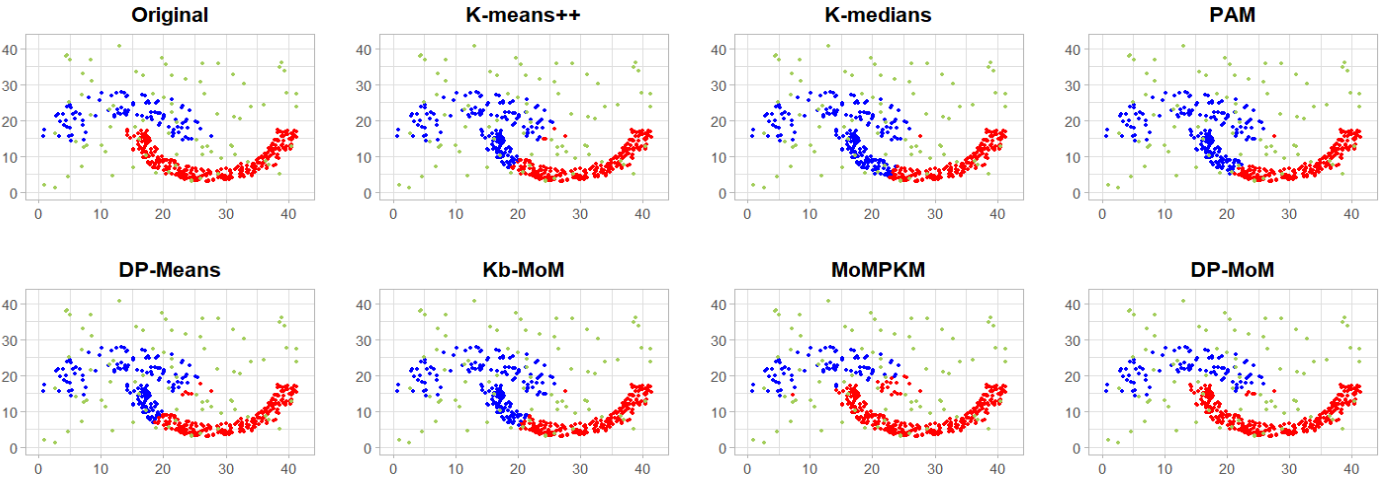
\includegraphics[width = \textwidth]{Diagrams/plot-jain-sim-comparison-0.7.png}
    \caption{Several state-of-the-art clustering methods fail to achieve proper clustering in presence of noisy observations (light green in color), while the performance of DP-MoM, our proposed algorithm, is nearly optimal.}
    \label{fig:jain-out}
\end{figure*}

Bayesian approaches generally offer room for flexible models in various settings, for instance when the number of clusters is unknown. Among these methods, there are two prominent existing approaches. One of them is to assume a Poisson prior on the number of clusters. The  other one is the Dirichlet process mixture model \citep{hjort_holmes_müller_walker_2010}, a Bayesian nonparametric model, which gives rise to infinite mixture models. Under certain conditions, it has been shown to possess some desirable properties such as consistency for the number of clusters \citep{ascolani-DP}. \citet{DP-Means} considered such an approach that bridges the concepts of $k$-means and Gaussian mixture models \citep{murphy2018machine}. Nevertheless, their method, called DP means, exhibits flexibility in guessing an optimal number of clusters; the algorithm utilizes the mean of the data points within the cluster for centroid updation, compromising its performance specifically on noisy or outlier-laden datasets.

% \begin{figure*}[t]
%     \centering
%     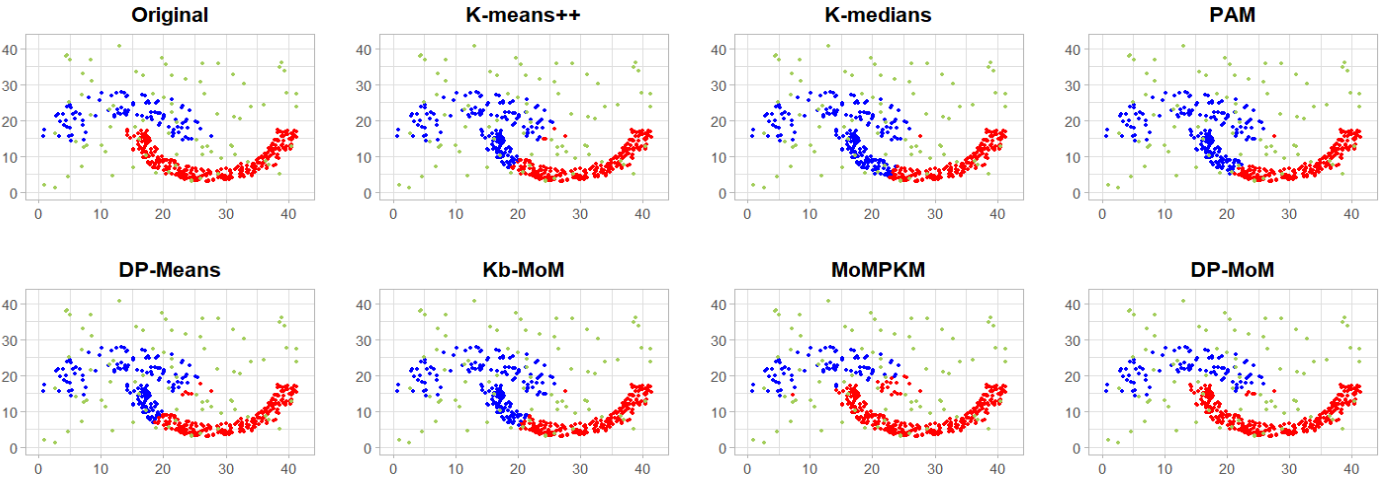
\includegraphics[width = \textwidth]{Diagrams/plot-jain-sim-comparison-0.7.png}
%     \caption{Several state-of-the-art clustering methods fail to achieve proper clustering in presence of noisy observations (light green in color), while the performance of DP-MoM, our proposed algorithm, is nearly optimal.}
%     \label{fig:jain-out}
% \end{figure*}

In this article, we tackle all these challenges by integrating two prominent clustering methodologies: centroid-based and model-based. Our proposed algorithm, DP-MoM, is designed to excel in scenarios with noisy or outlier-affected data, thanks to its use of the Median-of-Means (MoM) estimator \citep{nemirovsky1983wiley,devroye-MoM}. Moreover, it offers the advantage of not requiring a predefined number of clusters. To illustrate the efficacy of our approach, we provide a compelling example. We introduce randomly generated noisy observations into the \textit{Jain} dataset \citep{jain-dataset} (see Section \ref{sec:experiments} for more details) and then apply various state-of-the-art algorithms, including our proposed DP-MoM, to assess their performances on the original dataset. As depicted in Fig. \ref{fig:jain-out}, DP-MoM demonstrates notably superior clustering accuracy compared to existing algorithms.

\section{Background}
\label{gen_inst}

\subsection{Clustering based on Dirichlet Process}

\citet{DP-Means} proposed a method via Gibbs sampling, serving as a Bayesian counterpart to representing $k$-means with a mixture of Gaussians. We assume the following model to capture the cluster structure of the dataset whose limiting case reduces to the Dirichlet Process Mixture models:

\begin{align*}
\boldsymbol{\theta}_1, \ldots, \boldsymbol{\theta}_{{k}} & \sim {G}_0, \\
\pi & \sim \operatorname{Dir}\left({k}, \pi_0\right), \\
{z}_1, \ldots, {z}_{{n}} & \sim \operatorname{Discrete}(\pi), \\
{\bX}_1, \ldots, {\bX}_{{n}} & \sim \mathcal{N}\left(\boldsymbol{\theta}_{{z}_{{i}}}, \sigma I\right),
\end{align*}

% \begin{align*}
% \boldsymbol{\theta}_1, \ldots, \boldsymbol{\theta}_{{k}} \sim {G}_0~;~
% \pi \sim \operatorname{Dir}\left({k}, \pi_0\right)~;~
% {z}_1, \ldots, {z}_{{n}}  \sim \operatorname{Discrete}(\pi)~;~
% {\bX}_1, \ldots, {\bX}_{{n}} \sim \mathcal{N}\left(\boldsymbol{\theta}_{{z}_{{i}}}, \sigma I\right),
% \end{align*}
where $\boldsymbol{\theta}_{{j}}$ 's are the cluster centroids; ${G}_0$ is taken to be a $\mathcal{N}(0, \rho \mathbf{I})$ prior where $\mathbf{I}$ denotes the identity matrix of appropriate order. $\operatorname{Dir}\left({k}, \pi_0\right)$ denotes a Dirichlet distribution, where $\pi$ is the mixture probability with $\pi_0=\frac{\alpha}{k} \mathbf{1}$. Here, $\mathbf{1}$  denotes the vector (of appropriate order) of all $1$'s. For $i = 1,2,\ldots,n$, ${z}_{{i}}$ denotes the label assigned to the data points ${\bX}_{{i}}$, and  $\operatorname{Discrete}(\pi)$ indicates that ${z}_{{i}}$ takes the value $j$ with probability $\pi_{{j}}$, for ${j}=1, \ldots, {k}$.

The hard clustering algorithm, called \textit{DP-means}, proposed by \citet{DP-Means} is essentially the case when $\sigma \to 0$. This limiting case boils down to minimizing the objective:

\begin{equation}\label{dp-means-obj}
    f_{\operatorname{DP}} (\bTheta, k)=\sum_{i=1}^n \min _{1 \leq j \leq k}\left\|{\bX}_i-\boldsymbol{\theta}_j\right\|_2^2+\lambda k.
\end{equation}

The minimization of the function in \eqref{dp-means-obj} with respect to $k$ is performed iteratively. The distance from each data point to its closest cluster centroid is determined at each step of the algorithm. Subsequently, each point is assigned to the cluster with the nearest centroid unless this distance exceeds $\lambda$. In such an instance, a new cluster is initialized with the data point serving as the centroid of the newly created cluster. This algorithm determines the number of clusters in a dataset without necessitating prior knowledge of $k$. It maintains the simplicity inherent in Lloyd's approach while ensuring effectiveness even in situations where the actual number of clusters is unknown.


\subsection{Median-of-Means (MoM)}

Let us consider a simple scenario first where we observe $\bX_1,\bX_2,\ldots,\bX_n\sim F$ with a goal to estimate the mean of the distribution $F$, i.e., $\mu_0=\mathbb{E} [\bX_1]=\int x\,dF(x)$.

We employ the median-of-means (MoM) estimator to estimate $\mu_0$ as follows: Assume that the sample size $n=bL$ where $L$ is the number of buckets (subsamples) and $b$ is the size of each bucket. We first split the data randomly into $L$ partitions (or buckets) and calculate the mean of the data points belonging to each partition. This gives rise to estimators $\hat{\mu}_1,\hat{\mu}_2,\ldots,\hat{\mu}_L$. The MoM estimator defined to be the median of these $b$ many mean estimators, namely, $\hat{\mu}_{\text{MoM}}=\operatorname{median} (\hat{\mu}_1,\hat{\mu}_2,\ldots,\hat{\mu}_L).$

% \begin{equation}\label{MoM-defn}
% \hat{\mu}_{\text{MoM}}=\operatorname{median} (\hat{\mu}_1,\hat{\mu}_2,\ldots,\hat{\mu}_L).
% \end{equation}

In centroid-based clustering, the median-of-means estimator is used as follows: We first partition the dataset into $L$ subparts. In each iteration, we calculate the mean objective function value for each bucket $l$, $\frac{1}{b}\sum_{i \in B_{l}}f_{{\Theta}}(\bX_i)$ (where $\Theta$ is the collection of centroids from the previous iteration) and choose the bucket $L_t$ in such a way that
\begin{equation}\label{eq4}
    \sum_{i \in B_{L_t}}f_{{\bTheta}}(\bX_i)=\operatorname{median}_{l \in \{1,\ldots,L\}}\left\{\sum_{i \in B_{l}}f_{{\bTheta}}(\bX_i)\right\}.
\end{equation}
The centroids $\Theta$ are recalculated based on the observations in the bucket $B_{L_t}$ and all the observations are clustered using these centroids.

\begin{comment}
A reason why this estimator is of such interest (apart from being a robust estimator) is that given $\operatorname{var}(\bX_1)=\sigma^2<\infty$ in the finite sample case, it satisfies the following concentration inequality \citep{lerasle2019lecture}: 
\begin{equation}
    P(|\hat{\mu}_\text{MoM}-\mu_0| > \epsilon) \leqslant e^{-2L} \left(\frac{1}{2}-\frac{L}{n}\frac{\sigma^2}{\epsilon^2}\right)^2 \text{for all } n=bL.
\end{equation}
\end{comment}


\section{Dirichlet Process Clustering with MoM}

\subsection{Problem Formulation}
The problem posed to us is that of partitioning a given dataset $\mathcal{X} = \{\bX_1, \bX_2, \ldots, \bX_n\}\subset \mathbb{R}^p$ into natural, disjoint clusters such that the variance within each cluster is minimized at the same time maximizing the inter-partition variability. 


In centroid-based clustering, the $j^{th}$ cluster is represented by its centroid $\boldsymbol{\theta}_j$. The concept of ``closeness" is quantified through some divergence, which we shall consider to be the Euclidean distance, generated by $d(\boldsymbol{a},\boldsymbol{b})=\|\boldsymbol{a} - \boldsymbol{b}\|_2^2$. Prior knowledge of the number of centroids $k$ enables us to accomplish clustering by minimizing the objective
\begin{equation}\label{ob}
    f_{\boldsymbol{\Theta}}(\boldsymbol{X}) := \frac{1}{n} \sum_{i=1}^n \Psi\left(d_\phi\left(\boldsymbol{X}_i, \boldsymbol{\theta}_1\right), \ldots, d_\phi\left(\boldsymbol{X}_i, \boldsymbol{\theta}_k\right)\right).
\end{equation}

Here, $\Psi: {\mathbb{R}^{+}_0}^k \rightarrow \mathbb{R}^{+}_0$ is the function $\min_{1\le j\le k} d(\bm{X},\bm{\theta}_j)$. In our case, we will seek to minimize with respect to both $\{\bm{\theta_j}\}_{1\le j\le k}$ and $k$, the following objective function:
\begin{equation}\label{obj}
    \operatorname{median}\left(\frac{1}{b} \sum_{i \in B_1} f_{\boldsymbol{\Theta}}\left(\boldsymbol{X}_i\right), \ldots, \frac{1}{b} \sum_{i \in B_L} f_{\boldsymbol{\Theta}}\left(\boldsymbol{X}_i\right)\right) + \lambda k.
\end{equation}


\begin{comment}
\subsection{Optimization}

Optimizing the above objective is achieved using gradient-based methods. In our case, we employ the \textit{AdaGrad} algorithm \citep{duchi2011adaptive} for the said purpose. The centroids are updated as follows:
\begin{equation}
    \boldsymbol{\theta_j}^{(t+1)} := ~\boldsymbol{\theta}_j^{(t)} - \dfrac{\eta}{\sqrt{\varepsilon + \sum_{t' = 1}^t ||g_j^{(t')}||^2}} \cdot g_j^{(t)},
\end{equation}
where 
\begin{equation}
    g_j^{(t)} = \frac{1}{b}\sum_{i \in B_{l_t}} 2(\boldsymbol{\theta}_j^{(t)} - \bX_i)\cdot \mathbf{I}_{\{\bX_i \in \mathcal{C}_j\}}
\end{equation}
with $\mathbf{I}_{\{\bX_i \in \mathcal{C}_j\}}$ taking the value $1$ if $u_{ij}=1$ and $0$ otherwise.
\end{comment}


\subsection{Algorithm}

\begin{breakablealgorithm}%[!htb]
\vspace{-2mm}
\caption{Dirichlet Process Clustering using Median-of-Means (DP-MoM)}
\label{algo1}
\flushleft{
% \vspace{-2mm}
\textbf{Data}: Data matrix $\mathcal{X}$, Penalty parameter $\lambda$, $\epsilon$, Learning Rate $\eta$, Tolerance $\delta$.\\
\textbf{Result}: Number of clusters $k$, Cluster assignments $\mathcal{U}$, Cluster centroids $\bTheta$.\\
\textbf{Initialization}: Randomly divide $\{1,\dots,n\}$ into $L$ buckets of equal size. 
Set $\boldsymbol{\theta_1}=\frac{1}{n}\sum_{i = 1}^{n} \bX_i$, $k=1$, $b=\frac{n}{L}$, and $\mathcal{U}=\mathbf{1}$.\\
}
\vspace{2mm}
\begin{algorithmic}[1]
% \SetAlgoLined
 \While{$t<t_{\text{max}}$ \text{or stopping condition is not satisfied}}
  % instructions\;
  \For{every observation $\bX_i$}
  \State Compute $a_i$= $\min\left\{\|\bX_i - \boldsymbol{\theta_j}\|^2,~j = 1,\cdots,k\right\}$
  \If{$a_i > \lambda$}
  \State Set $k=k+1$, $\btheta_k=\bX_i$
  \State Update $\mathcal{U}$ by $u_{ij} = \delta\left(i=j\right)$  ~~[$\delta(A)$ represents the indicator of the event $A$]
% \ENDIF
   \Else
   \State Update $\mathcal{U}$ by $u_{ij}= \delta\left(j=\argmin_{1\leq c\leq k} ||\bX_i - \boldsymbol{\theta_c}||^2\right)$
   \EndIf
   \EndFor
  \State Find $l_t \in \{1, 2, ... , L\}$ such that $\displaystyle\frac{1}{b}\sum_{i \in B_{l_t}} f_{\boldsymbol{\Theta^{(t)}}}(\bX_i) = \displaystyle\operatorname{median}_{1\leqslant j\leqslant L} \left\{\displaystyle \frac{1}{b}\sum_{i \in B_{j}}f_{{\bTheta}}(\bX_i)\right\}$
  \State For each $j\in \{1, 2, ..., k\}$: $\displaystyle g_j^{(t)} = \displaystyle\frac{1}{b}\sum_{i \in B_{l_t}} 2(\boldsymbol{\theta}_j^{(t)} - \bX_i)u_{ij}$
  \State Update ${\Theta}$ by $\displaystyle\boldsymbol{\theta}_j^{(t+1)} := ~\boldsymbol{\theta}_j^{(t)} - \dfrac{\eta}{\sqrt{\varepsilon + \sum_{t' = 1}^t ||g_j^{(t')}||^2}} \cdot g_j^{(t)}$
 \EndWhile
\end{algorithmic}
\end{breakablealgorithm}

% $$\text{THE ALGORITHM WILL BE STATED HERE}$$

Algorithm \ref{algo1} summarizes the pseudocode for our procedure. The objective function is optimized using the \textit{AdaGrad} algorithm \citep{duchi2011adaptive}. We chose \textit{AdaGrad} over commonly used optimizers like \textit{Adam} \citep{Kingma2015Adam}  because it yielded better results in most of our clustering use cases, though we do not include these results to maintain readability. In addition, by scaling the gradients of each parameter using the past gradients\textit{AdaGrad} avoids the issues of vanishing and exploding gradients \citep{pmlr-v97-ward19a}, especially for sparse data that frequently appears in our high-dimensional use cases. The choice of the values of the tuning parameters is discussed in the Appendix.

\begin{comment}
\subsection{Parameter Selection}
The first step in our proposed algorithm is partitioning the dataset randomly. This is achieved by choosing a permutation of the data points uniformly and then placing them in different buckets in the order of the permutation. Though this technique achieves randomness in terms of partitioning the data, arbitrary partitioning may lead to undesirable results, which is why the partitioning (or permutation for that matter) needs to be carefully chosen. We resort to a form of grid search to solve this problem. We determine $\lambda_{\min}$ and $\lambda_{\max}$, the minimum and maximum pairwise squared distance between the data points, respectively. $11$ equally-spaced points $\lambda_{\min} =\lambda^1_1<\lambda^1_2< \cdots < \lambda^1_{10}<\lambda^1_{11}=\lambda_{\max}$ are picked, and the algorithm is run for these values and for all values of number of partitions, $L$, such that $2<L<\frac{n}{3}$. We select $\lambda^1_{i^*}$ corresponding to the most accurate clustering and divide its neighborhood $[\lambda^1_{i^*-1},\lambda_{i^*-1}]$  $\left([\lambda^1_1,\lambda^1_2]\operatorname{ or }[\lambda^1_{10}, \lambda^1_{11}]\right)$ into $20$ divisions and re-run the algorithm as we did in the interval $[\lambda_{\min}, \lambda_{\max}]$. We repeat this one more time, so that the feasible range for the penalty parameter $\lambda$ has been segmented to the order of $10^3$. We obtain the permutation corresponding to the most accurate clustering in the 3 stages above, and use this particular permutation to partition the data for further experiments.

We imitate the above experiment, except that this time we use the permutation of the data points that have been obtained from the said grid-searching, to partition the data. We then choose the $\lambda$ and $L$ values for which the best clustering accuracy is attained. We call them $\lambda_{opt}$ and $L_{opt}$. Since our proposed algorithm is a randomized one, we cannot readily conclude that $\lambda_{opt}$ and $L_{opt}$ are the only values corresponding to which we will obtain high clustering accuracy. In fact, for another repetition of the above experiment, we may not obtain an identical favorable permutation or the same optimal $\lambda$ and $L$ values. So, we repeat the aforementioned grid-searching experiment a number of times (say about 30 times) so that we may obtain a range of $\lambda$ and a range of $L$ that will be suitable to work with in order to derive the best results out of the proposed framework. We choose the median of the clustering accuracies, measured with the Adjusted Rand Index (ARI) \citep{Hubert1985} so obtained, as a representative of the clustering accuracy of the algorithm.
\end{comment}

\subsection{Computational Complexity}
% \textcolor{red}{$\mathcal{O}(nKp)$ per iteration}
In each iteration, our algorithm first ascertains whether an increase in the number of clusters is needed. The centroids are recalculated thereafter, and the cluster assignments are made accordingly. This phase typically takes $\mathcal{O}(nCp)$ time steps to complete, where $C$ represents the number of clusters in that iteration. The calculations presented in the following section assume that the number of clusters is upper bounded by some finite $K<n$. Consequently, the worst case runtime of the DP-MoM algorithm remains $\mathcal{O}(nKp)$ for every iteration.

The computational complexity of the DP-means algorithm is comparable to that of DP-MoM, as each iteration requires $\mathcal{O}(nCp)$ steps to complete, with $C$ denoting the number of clusters in that specific iteration. On the contrary, $k$-means demands $\mathcal{O}(nkp)$ steps per iteration, with $k$ representing the predefined cluster count. This is typically slated to be lower than that of DP-means or DP-MoM. In the case $k=K$, however, $k$-means will perform no better than DP-MoM in terms of runtime.


\section{Theoretical Results}
\label{sec:theory}

% We seek to minimize the objective function (\ref{obj}) with the assumption that we will stop updating the clusters when the total number of clusters reach a maximum value of $K$. Then we can derive the finite sample error bounds for the method, similar to \citep{paul2021uniform}. 

% \begin{assumption}\label{a1}
% $\bX_1\dots,\bX_n \overset{i.i.d.}{\sim} P$ such that $P \in \mathcal{M}$.
% \end{assumption}

% \begin{assumption}\label{a2}
%     The number of clusters $k$ is bounded above by some positive constant $K$, where $K<n$.
% \end{assumption}

% Let $P_n$ denote the empirical distribution derived from the data $\bX_1\ldots,\bX_n$. In other words, for any Borel set $A$, $P_n(A) = \frac{1}{n}\sum_{i=1}^n \mathbf{I}\{\bX_i \in A\}$. 
% To simplify notation, we use $\mu f := \int f d\mu$. 

% By utilizing the Strong Law of Large Numbers (SLLN) as presented in \citep{athreya2006measure}, we can conclude that $P_n f_{\bTheta}$ converges almost surely to $Pf_{\bTheta}$, where the objective \ref{obj} can be reformulated as a constrained minimization, 


% \begin{equation}
%     \operatorname{median}\left(\frac{1}{b} \sum_{i \in B_1} f_{\boldsymbol{\Theta}}\left(\boldsymbol{X}_i\right), \ldots, \frac{1}{b} \sum_{i \in B_L} f_{\boldsymbol{\Theta}}\left(\boldsymbol{X}_i\right)\right),\quad\text{subject to, } k\leq K.
% \end{equation}


Let us denote the set of all probability measures $P$ with support on $[-M,M]^p$ by $\mathcal{M}$%, i.e., $P\left([-M,M]^p\right)=1$ $\forall$ $P\in \mathcal{M}$
. We shall make a standard assumption that all the data points are independent and identically distributed (\textit{i.i.d.}) with bounded components.

\begin{assumption}\label{ass-1-iid}
    $\bm{X}_1,\bm{X}_2,\ldots,\bm{X}_n \overset{\text{iid}}{\sim}P$ such that $P\in \mathcal{M}$.
\end{assumption}

We denote the empirical distribution derived from $\bX_1\ldots,\bX_n$, by $P_n$, that is, $P_n(A) = \frac{1}{n}\sum_{i=1}^n \mathbf{I}\{\bX_i \in A\}$ for any Borel set $A$. 
For the sake of notational simplicity, we write $\mu f := \int f \, d\mu$. Thanks to the Strong Law of Large Numbers (SLLN) presented in \citep{athreya2006measure}, we can conclude that $P_n f_{\bTheta} \rightarrow Pf_{\bTheta}$ almost surely. Let $\widehat{\bm{\Theta}}_n$ be a minimizer of \[f_{\bm\Theta}(\bm{X})=\frac{1}{n} \sum_{i=1}^n \Psi(d(\bm{X}_i, \bm{\theta}_1), \ldots, d(\bm{X}_i, \bm{\theta}_k)),\]
and $\bm{\Theta}^*$ be the global minimizer of $Pf_{\bm{\Theta}}$. 
Owing to the fact that $P_n f_{\bm{\Theta}}$ and $P f_{\bTheta}$ are close for large enough $n$, it is reasonable to expect that the absolute difference between $\widehat{\bm{\Theta}}_n$ and $\bm{\widehat{\Theta}}^*$ will be small. %To show that $\bm{\widehat{\Theta}}_n$ converges to $\bm{\Theta}^*$ as $n\to \infty $, we consider bounding the uniform deviation $\sup_{\bm{\Theta}}|P_n f_{\bm{\Theta }}-Pf_{\bm{\Theta}}|$.

\begin{assumption}\label{ass-2-cluster-count}
    The number of clusters $k$ is bounded above by some finite $K\in \mathbb{N}$, where $K < n$.
\end{assumption}

The inherent dependency of the number of centroids on the cluster penalty parameter $\bm{\lambda}$ makes it possible for us to choose $\bm{\lambda}$ appropriately so that the cluster count doesn't exceed $K$. Moreover, we deduce from A\ref{ass-2-cluster-count} that, at a certain juncture, the number of centroids reaches a state of stability. In this state, it is only the cluster centroids themselves that undergo updates during each iteration, while the number of centroids remains constant. This will make our analysis independent of the penalty parameter $\bm{\lambda}$ as the term $k\bm{\lambda}$ is not subject to change after a finite number of iterations. Consequently, beyond a finite number of steps, the objective function effectively reduces to 
\begin{equation}\label{DP-MoM-obj}
    \operatorname{MoM}_L^n(\bTheta) := \operatorname{median} \left(\frac{1}{b}\sum_{i\in B_{1}}f_{\bm{\Theta}}(\bm{X}_i), \ldots, \frac{1}{b}\sum_{i\in B_{\ell}}f_{\bm{\Theta}}(\bm{X}_i)\right).
\end{equation} 

\begin{remark}
    In our framework, $\displaystyle |\Psi(\bm{x})-\Psi(\bm{y})|\le \|\bm{x}-\bm{y}\|_1$.
\end{remark}

To see this, recall the definition of $\Psi$ in \eqref{obj}, and note that $|\Psi(\bm{x})-\Psi(\bm{y})|=|\min_{1\le j\le K}x_j-\min_{1\le j\le K}y_j|$. Let us assume, without loss of generality, that $\min_{1\le j\le K}x_j\ge \min_{1\le j\le K}y_j$. Hence, $\min_{1\le j\le K}x_j-\min_{1\le j\le K}y_j\le x_{j^*}-y_{j^*}\le \|\bm{x}-\bm{y}\|_1$ where $j^* = \operatorname{argmin}_{1\le j\le K}y_j$.

% \begin{lemma}\label{lemma-a1-lipschitz}
%     For $\bm{x},\bm{y}\in [-M,M]^p$, $\phi(\bm{u})=\|\bm{u}\|_2^2$ is $2M\sqrt{p}$-Lipschitz i.e. \[|\phi(\bm{x})-\phi(\bm{y})|\le 2M\sqrt{p}\|\bm{x}-\bm{y}\|_2\]
% \end{lemma}


% Then it is equivalent to solving the unconstrained minimization problem with $K$ many clusters. Hence,
% \begin{equation}
%     P_nf_{\bTheta}=\operatorname{median}\left(\frac{1}{b} \sum_{i \in B_1} f_{\boldsymbol{\Theta}}\left(\boldsymbol{X}_i\right), \ldots, \frac{1}{b} \sum_{i \in B_L} f_{\boldsymbol{\Theta}}\left(\boldsymbol{X}_i\right)\right)
% \end{equation}

% Thus, the optimization problem becomes equivalent to MoMPKM \citep{paul2021uniform}. Thus, under the same assumptions $A1-A6$ of \citep{paul2021uniform}, for a fixed number of features $p$, with probability at least $1-\delta$ for some $\delta>0$, the following holds.
% \begin{equation}
%     |Pf_{\hat{\bTheta}_n} - P f_{\bTheta^\ast}|  \le 192 \sqrt{\pi} \tau_{\balpha, K} H_p M^2  (Kp)^{3/2} n^{-1/2} + 8 \tau_{\balpha, K} H_p M^2 p K \sqrt{\frac{\log(2/\delta)}{2n}}.
% \end{equation}
% Here, $\hat{\bTheta}_n$ is the empirical minimizer, $\bTheta^\ast$ is the global population minimizer, $\tau_{\balpha, K}$ is a Lipschitz constant for the function $\Psi_\alpha$ defined in (\ref{psi}), $M$ is a positive constant which comes from the assumption that $\bTheta^\ast \in \mathscr{G}$. 

% \begin{remark}
% For constant $p$ and $K$, the finite sample error rate becomes $O_P (n^{-1/2})$. Also, in this case, $\hat{\bTheta}_n \xrightarrow{a.s.} \bTheta^\ast$. 
% \end{remark}
% \begin{remark}
%     If $K$ varies and is of the order $\log n$, then the error rate becomes $\mathcal{O}_P\left(\sqrt{(\log n)^3/n}\right)$.
% \end{remark}
% If $K$ varies, for fixed $p$, the error bound is $\mathcal{O}_P\left(\sqrt{K^3/n}\right)$. Thus, for the error to asymptotically go to zero, we must have $K$ such that $\lim_{n\rightarrow \infty} \frac{K^3}{n} = 0$. In general, for varying $p$, the finite sample error bound is $\mathcal{O}_P((Kp)^{3/2}n^{-1/2})$, hence we must have $\lim_{n\rightarrow \infty} \frac{(Kp)^3}{n} = 0$.

% \begin{lemma}\label{lemma-a2}
%     Under A\ref{ass-1-iid} and A\ref{ass-2-cluster-count}, for any $\bm{\Theta}, \bm{\Theta'}\in [-M,M]^p$, \[\|f_{\bm{\Theta}} - f_{\bm{\Theta'}}\|_{\infty}\le 4M\sqrt{p}\sum_{j=1}^{K}\|\bm{\theta}_j-\bm{\theta}_j'\|_2\]
% \end{lemma}


% \subsection{Bounding the minimizers \texorpdfstring{$\widehat{\bm{\Theta}}_n$}{theta-hat-n} and \texorpdfstring{$\bm{\Theta}^*$}{theta-star}}

\subsection{Concentration Inequalities on the Empirical Measure through Rademacher Complexity}

We start off by defining $\mathscr{G} := [-M,M]^{K \times p}$. To show that $\displaystyle \widehat{\bm{\Theta}}_n$ converges to $\bm{\Theta}^*$ as $n \to \infty$, the first step is to prove that both $\widehat{\bm{\Theta}}_n$ and $\displaystyle \bm{\Theta}^*$ lie in $\mathscr{G}$. We begin with the following result.

% \begin{lemma}\label{lemma-1-obtuse}
%     Let $\mathcal{C}$ be a convex set, and suppose $P_{\mathcal{C}}(\bm{\theta})$ be the projection of $\bm{\theta}$ onto $\mathcal{C}$, with respect to the Bregman divergence $d(\cdot,\cdot)$ i.e. $P_{\mathcal{C}}(\bm{\theta})=\operatorname{argmin}_{\bm{x}\in \mathcal{C}}d(x,\bm{\theta})$ (assuming it exists). Then \[d(\bm{x}, \bm{\theta})\ge d(\bm{x}, P_{\mathcal{C}(\bm{\theta})})+d(P_{\mathcal{C}(\bm{\theta})}, \bm{\theta})\hspace{0.3cm}\text{ for all }\bm{x}\in \mathcal{C}.\]
% \end{lemma}

\begin{lemma}\label{lemma-1-obtuse}
    Consider a convex set $\mathcal{C}$ and let $P_{\mathcal{C}}(\bm{\theta})$ be the projection of $\bm{\theta}$ onto $\mathcal{C}$ with respect to $d(\bm{x},\bm{\theta})=\|\bm{x}-\bm{\theta}\|_2^2$, i.e., $P_\mathcal{C}(\bm{\theta})=\operatorname{argmin}_{\bm{x}\in \mathcal{C}}\|\bm{x}-\bm{\theta}\|_2^2$. Then \[\|\bm{x}-\bm{\theta}\|_2^2\ge \|\bm{x}-P_{\mathcal{C}}(\bm{\theta})\|_2^2+\|P_{\mathcal{C}}(\bm{\theta})-\bm{\theta}\|_2^2.\]
\end{lemma}

Lemma \ref{lemma-1-obtuse} follows directly from the obtuse angle property presented in Section 3 of \citep{paul2021a}, by setting $d_\phi$ to be the squared Euclidean distance. We next show that for minimizing $P_n f_{\bm{\Theta}}$ or $P f_{\bm{\Theta}}$, it is enough to restrict our search space to $\mathscr{G}$.

\begin{lemma}\label{lemma-2}
    Let $Q \in \mathcal{M}$. For any $\bm{\Theta} \in \mathbb{R}^{K \times p}$, there exists $\bm{\Theta}^{\prime} \in\mathscr{G}$, such that $Q f_{\bm{\Theta^{\prime}}} \leq Q f_{\bm{\Theta}}$.
\end{lemma}

Since we can restrict our attention to $\mathscr{G}$ to minimize $Q f_{\bm\Theta}$, we have the following:

\begin{cor}
    Let $Q \in \mathcal{M}$. If $\bm{\Theta}_0=\argmin_{\bm{\Theta} \in \mathbb{R}^{K \times p}} \int f_{\bm{\Theta}} \,dQ$, then $\bm{\Theta}_0 \in \mathscr{G}$.
\end{cor}

Note that under A\ref{ass-1-iid} and A\ref{ass-2-cluster-count}, both $P$ and $P_n$ have support contained in $\mathscr{G}$. Corollary \ref{cor-4.2} follows from the preceding by replacing $Q$ by $P$ and $P_n$.

\begin{cor}\label{cor-4.2}
    Under A\ref{ass-1-iid}--A\ref{ass-2-cluster-count}, both $\widehat{\boldsymbol{\Theta}}_n, \boldsymbol{\Theta}^* \in \mathscr{G}$.
\end{cor}

%Now that we have bounded $\widehat{\bm{\Theta}}_n$ and $\bm{\Theta}^*$ in a compact set, the following section supplies probabilistic bounds on the uniform deviation $2 \sup _{\bm{\Theta} \in\mathscr{G}}\left|P_nf_{\bm\Theta} - Pf_{\bm{\Theta}}\right|$ via metric entropy arguments.


% \subsection{Concentration Inequality and Metric Entropy Bounds via Rademacher Complexity}

%We have proven that $\widehat{\boldsymbol{\Theta}}_n, \boldsymbol{\Theta}^* \in\mathscr{G}$. 


% \begin{align*}
%     |P f_{\widehat{\bm{\Theta}}_n}- P f_{\bm{\Theta^*}}|
%     = P f_{\widehat{\bm{\Theta}}_n}- P f_{\bm{\Theta^*}} 
%     &= P f_{\widehat{\bm{\Theta}}_n}-P_n f_{\widehat{\bm{\Theta}}_n}+P_n f_{\widehat{\bm{\Theta}}_n}-P_n f_{\bm{\Theta^*}}+P_n f_{\bm{\Theta^*}} - P f_{\bm{\Theta^*}}\\
%     &\le P f_{\widehat{\bm{\Theta}}_n}-P_n f_{\widehat{\bm{\Theta}}_n}+P_n f_{\bm{\Theta^*}} - P f_{\bm{\Theta^*}}\\
%     &\le 2\sup_{\bm{\Theta}\in \mathscr{G}}|P_n f_{\bm\Theta}-P f_{\bm\Theta}|
% \end{align*}


Towards bounding $|P f_{\widehat{\bm{\Theta}}_n}-P f_{\bm{\Theta}^*}|$, it suffices to bound the quantity $\sup _{\bm{\Theta} \in\mathscr{G}}\left|P_n f_{\bm\Theta} - P f_{\bm\Theta}\right|$, since
% Next, we observe that
\begin{align*}
    |P f_{\widehat{\bm{\Theta}}_n}- P f_{\bm{\Theta^*}}| 
    = P f_{\widehat{\bm{\Theta}}_n}-P f_{\bm{\Theta^*}} \le P f_{\widehat{\bm{\Theta}}_n}-P_n f_{\widehat{\bm{\Theta}}_n}+P_n f_{\bm{\Theta^*}} - P f_{\bm{\Theta^*}}\le 2\sup_{\bm{\Theta}\in \mathscr{G}}|P_n f_{\bm\Theta}-P f_{\bm\Theta}|.
\end{align*}

Employing Rademacher complexity \citep{DUDLEY1967290,FoML-mohri}, we constrain this deviation and subsequently establish an upper bound on it. Let $\mathcal{F}=\left\{f_{\bm\Theta}: \bm{\Theta} \in\mathscr{G}\right\}$. Also, define the $\mathcal{F}$-norm $\|\mu-\nu\|_{\mathcal{F}}$ between two probability measures $\mu$ and $\nu$ \citep{athreya2006measure} by $ \sup_{f \in \mathcal{F}}\left|\int f \,d\mu-\int f \,d\nu\right|$. Recall that the Rademacher complexity is defined as follows:

\begin{defn}
    (Rademacher complexity) Let $\epsilon_i$'s be i.i.d. Rademacher random variables independent of $\mathcal{X}=\left\{\boldsymbol{X}_1, \ldots, \boldsymbol{X}_n\right\}$, i.e. $\mathbb{P}\left(\epsilon_i=1\right)=\mathbb{P}\left(\epsilon_i=-1\right)=0.5$. Population Rademacher complexity of $\mathcal{F}$ is defined as $\mathcal{R}_n(\mathcal{F})=\E\sup _{f \in \mathcal{F}} \frac{1}{n} \sum_{i=1}^n \epsilon_i f\left(\boldsymbol{X}_i\right)$, where the expectation is over both $\epsilon$ and $\mathcal{X}$.
\end{defn}

\begin{comment}
\begin{defn}
    ($\delta$-cover and Covering Number) Let $(X, d)$ be a metric space. The set $X_\delta \subseteq X$ is said to be a $\delta$-cover of $X$ if for all $x \in X, \exists$ $x^{\prime} \in X_\delta$, such that $d\left(x, x^{\prime}\right) \leq \delta$. The $\delta$-covering number of $X$ w.r.t. $d$, denoted by $N(\delta ; X, d)$, is the size of the smallest $\delta$-cover of $X$ with respect to $d$.
\end{defn}

The following lemma gives a bound for the $\delta$-covering number of $\mathcal{F}$ under the supremum norm. The main idea here is to use the Lipschitz property of $f_{\Theta}$ and then to find a cover of the search space for $\Theta$, i.e. $\mathscr{G}$. This then automatically transcends to a cover of $\mathcal{F}$ under the sup-norm.

\begin{lemma}\label{lemma-3-cov-num}
    Let $N\left(\delta ; \mathcal{F},\|\cdot\|_{\infty}\right)$ be the $\delta$-covering number of $\mathcal{F}$ under $\|\cdot\|_{\infty}$. Then, under  assumptions A\ref{ass-1-iid} and A\ref{ass-2-cluster-count}, $$N\left(\delta ; \mathcal{F},\|\cdot\|_{\infty}\right) \leq\left(\max \left\{\left\lfloor\frac{4 M^2 K p}{\delta}\right\rfloor, 1\right\}\right)^{Kp}.$$
\end{lemma}

\begin{lemma}\label{lemma-4-diam}
    Let diam($\mathcal{F}$)=$\sup_{f,g\in \mathcal{F}}\|f-g\|_{\infty}$. Then under A\ref{ass-1-iid} and A\ref{ass-2-cluster-count}, diam($\mathcal{F}$) $\le 8M^2Kp$.
\end{lemma}
\end{comment}

% Lemma \ref{lemma-4-diam} puts an upper bound on the diameter of $\mathcal{F}$, defined above, under $\|\cdot\|_{\infty}$. 
Following \citet{paul2021uniform}, we can devise a bound on the Rademacher complexity $\mathcal{R}_n(\mathcal{F})$.

\begin{thm}\label{thm-1-RnF}
    Under A\ref{ass-1-iid}--A\ref{ass-2-cluster-count}, 
    \begin{equation*}
        \mathcal{R}_n(\mathcal{F})\le 48\sqrt{\pi}M^2(Kp)^{3/2}n^{-1/2}.
    \end{equation*}
\end{thm}

% Before we proceed further, we would like to state the following lemma which puts a uniform bound on $\|f\|_{\infty}$ for $f\in \mathcal{F}$.
\begin{comment}
\begin{lemma}\label{lemma-5}
    For all $x\in [-M,M]^p$ and $\bm{\Theta}\in \mathscr{G}$, \[0\le \Psi(d(\bm{x},\bm{\theta}_1), d(\bm{x},\bm{\theta}_2),\cdots, d(\bm{x},\bm{\theta}_K) )\le 4M^2p.\]
\end{lemma}
\end{comment}

Given the result stated in Theorem \ref{thm-1-RnF}, we seek a non-asymptotic bound on $|P f_{\widehat{\bm{\Theta}}_n}-Pf_{\bm{\Theta}^*}|$ by deriving a uniform concentration inequality on $\|P_n-P\|_{\mathcal{F}}$.

\begin{thm}\label{thm-2-diff-Pn-P}
    Under A\ref{ass-1-iid}--A\ref{ass-2-cluster-count}, for any $\delta\in(0,1)$, the inequality 
    \[\|P_n-P\|_\mathcal{F}\le \left[96\sqrt{\pi}M^2(Kp)^{3/2} + 4\sqrt{2} M^2p\log^{\frac{1}{2}}\big(\tfrac{2}{\delta}\big) \right] n^{-1/2}\]
    holds with probability at least $1-\delta$.
\end{thm}

% The result in Theorem \ref{thm-2-diff-Pn-P} reveals a non-asymptotic bound on $|P f_{\widehat{\bm{\Theta}}_n}-Pf_{\bm{\Theta}^*}|$:

\begin{cor}
    Under A\ref{ass-1-iid}--A\ref{ass-2-cluster-count}, for any $\delta\in(0,1)$,% the following holds: 
    \begin{align*}
    |P f_{\widehat{\bm{\Theta}}_n}-Pf_{\bm{\Theta}^*}| &\le \Big[192\sqrt{\pi}M^2(Kp)^{3/2}+ 8\sqrt{2} M^2p\log^{\frac{1}{2}}\big(\tfrac{2}{\delta}\big) \Big] n^{-1/2}
    \end{align*}
    holds with probability at least $1-\delta$.
\end{cor}


\subsection{Asymptotic Properties: Strong Consistency and Rate of Convergence}

We now consider the classical setting where $p$ is held constant and demonstrate that the previously presented results imply strong consistency, with the rate of convergence of the order of $\mathcal{O}(n^{-1/2})$. We first follow the same idea of convergence of $\hth$ to $\bTheta^\ast$ that is outlined in \citep{pollard1981strong}. Since the centroids are unique up to the rearrangement of labels, our concept of dissimilarity
\[\mathcal{D}(\bTheta_1,\bTheta_2) = \min_{M \in \mathscr{P}_K} \|\bTheta_1 - M \bTheta_2\|_F \]
is considered over $\mathscr{P}_K$ the set of all real permutation matrices of order $K$, where $\|\cdot\|_F$ represents the
Frobenius norm. The sequence $\bTheta_n\to \bTheta$ if $\lim_{n\to \infty} \mathcal{D}(\bTheta_n,\bTheta)=0$. Following \citep{terada2014strong,chakraborty2020entropy}, we assume the identifiablity condition:

\begin{assumption}\label{ass-3-diss}
    $\forall$ $ \eta>0$, $\exists$ $\epsilon>0$, such that $\, \mathcal{D}(\bTheta,\bTheta^\ast)> \eta$ $\implies$ $P f_{\bTheta} > P f_{\bTheta^\ast} + \epsilon$ .
\end{assumption}

We now examine the strong consistency of $\hth$. In addition, we analyze the rate at which $|P f_{\hth} - P f_{\bTheta^\ast}|$ approaches $0$. Theorem \ref{thm-3-strong-consistency} affirms that strong consistency holds, with $\mathcal{O}(n^{-1/2})$ rate of convergence. Note that $X_n = \mathcal{O}_P(a_n)$ denotes that the sequence $X_n/a_n$ is bounded in probability.

\begin{thm}\label{thm-3-strong-consistency}
(Theorem 3.3 of \citep{paul2021uniform}) If $p$ is assumed to be constant then under  A\ref{ass-1-iid}--A\ref{ass-3-diss}, $\hth \xrightarrow{a.s.} \bTheta^\ast$ under $P$. Additionally, $|P f_{\hth} - P f_{\bTheta^\ast}| = \mathcal{O}_P (n^{-1/2})$.
\end{thm}


\subsection{Analysis under the Median-of-Means (MoM) Paradigm}

The results and analysis we have presented so far pertain to the situation where outlying or contaminating observations are absent. In this section, we assess the behavior of the centroids and the performance of Algorithm \ref{algo1} in the presence of outlying observations. %Without loss of generality, we assume $n=L\cdot B$. 
  We represent the set of all inliers as $\{\bX_i\}_{i \in \I}$ and the outliers as $\{\bX_i\}_{i \in \cO}$. Denoting the minimizer of \eqref{eq4} by $\tm$, we make the following assumptions for determining the rate at which $|Pf_{\tm} - Pf_{\bTheta^\ast}|$ approaches $0$. % as a function of $n,\,p,\,k,\,L$ and $|\I|$. To this end, 

\begin{assumption}\label{ass-4-iid}
    $\{\bX_i\}_{i \in \I}\sim P$ are i.i.d. with $P \in \mathcal{M}$.
\end{assumption}

\begin{assumption}\label{ass-5-L}
    $\exists$ $\, \eta > 0$ such that $L>(2+\eta)|\cO|$.
\end{assumption}

It is important to note that A\ref{ass-4-iid} is exactly the same as A\ref{ass-1-iid}, but specifically applied to the inliers. A\ref{ass-5-L} guarantees that at least half of the $L$ partitions are devoid of outliers; which is a milder requirement compared to the condition $L > 4|\cO|$ imposed in the recent work \citep{lecue2020robust}. Crucially, we highlight that no distributional assumptions are imposed on the outliers, permitting them to be unbounded, originate from heavy-tailed distributions, or exhibit any sort of dependence structure among each other. We cite Lemma 4.6 and subsequent Corollary 4.4 from \citep{paul2021uniform}.

\begin{lemma}\label{lemma-6-spmom}
Under A\ref{ass-4-iid}-A\ref{ass-5-L}, for any $\bTheta \in \Real^{K\times p}$, $\exists$ $\bTheta^\prime \in \mathscr{G}$, such that $\text{MoM}_L^n(\bTheta^\prime) \le \text{MoM}_L^n(\bTheta)$.
\end{lemma}

\begin{cor}
Under A\ref{ass-4-iid}-A\ref{ass-5-L}, $\tm \in \mathscr{G}$.
\end{cor}

The above results confirm that the search space for $\tm$ may be constrained to $\mathscr{G}$. Subsequently, we establish a bound on $\sup_{\bTheta \in \mathscr{G}} |\text{MoM}^n_L (f_{\bTheta}) - Pf_{\bTheta} |$, and further use it to bound $|P f_{\tm} - P f_{\bTheta^\ast}|$. 
We %define $\delta:=2/(4+\eta) - |\cO|/L$, and 
use ``$\lesssim$'' to denote the fact that a quantity is lesser than a constant multiple of the other. % $\delta:= \frac{2}{4+\eta} - \frac{|\cO|}{L}$; 


\begin{thm}\label{thm-4-MoM}
Under A\ref{ass-4-iid}-A\ref{ass-5-L}, with probability at least $1-4e^{-L \delta^2/2}$, 
\begin{align*}
    &\sup_{\bTheta \in \mathscr{G}} \left|\text{MoM}^n_L (f_{\bTheta}) - Pf_{\bTheta} \right|\lesssim  \max\left\{ Kp L^{1/2}n^{-1/2}, (Kp)^{3/2}  |\I|^{1/2}n^{-1}\right\}.
\end{align*}
\end{thm}

We present below a corollary that aids us in controlling the absolute difference $|P f_{\tm} - P f_{\bTheta^\ast}|$.

\begin{cor}
Under A\ref{ass-4-iid}-A\ref{ass-5-L}, with  probability at least $1-4e^{-L \delta^2/2}$,
\begin{align*}
    &\left|P f_{\tm} - P f_{\bTheta^\ast}\right|\lesssim \max\left\{ KpL^{1/2}n^{-1/2}, (Kp)^{3/2} |\I|^{1/2}n^{-1}\right\}.
\end{align*}
\end{cor}


\section{Experiments}
\label{sec:experiments}
We empirically validate our proposed clustering framework by implementing it on several datasets from the UCI Machine Learning Repository\footnote{\url{https://archive.ics.uci.edu/}} and the Compcancer database\footnote{\url{https://schlieplab.org/Static/Supplements/CompCancer/}} and then comparing it with existing approaches, utilizing the Adjusted Rand Index (ARI) for robust performance assessment. Our evaluation covers a range of centroid-based clustering methods, including $k$-means$++$, Sparse $k$-means (SKM) \citep{SKM-paper}, $k$-medians, Partition around Medoids (PAM) \citep{PAM-paper}, Robust Continuous Clustering (RCC) \citep{Shah2017-jj}, DP-means \citep{DP-Means}, $k$-bootstrap Median-of-Means ($k$b-MoM) \citep{brunetsaumard2020kbmom}, MoMPKM, and OWL $k$-means \citep{pmlr-v206-chakraborty23a}. These peers, representing state-of-the-art algorithms, are systematically compared against our proposed DP-MoM algorithm in diverse experimental scenarios. %Our first experiment involves testing the aforementioned techniques on several datasets from the UCI Machine Learning Repository\footnote{\url{https://archive.ics.uci.edu/}} and the Compcancer database\footnote{\url{https://schlieplab.org/Static/Supplements/CompCancer/}}.
Since our method relies on randomization while partitioning the data into buckets, the accuracy measure has been computed as the median of the obtained ARI over $31$ test runs. It was observed, for most of the datasets, that DP-MoM performed considerably better than its competitors in terms of ARI. Apart from this, 2 other experiments were conducted to assess the strength of the algorithm in terms of robustness and ability to detect clusters of various shapes that were in proximity to one another. The relevant source codes are available in the supplementary material. 


\subsection{Simulation Studies}
% \paragraph{Introducing Outliers in Real Data} \newline

\subsubsection{Study of Robustness on Simulated Data} $30$ data points are generated from each quadrant in the $2$-dimensional Euclidean plane using the following scheme. For the first quadrant, we generate $R_i \sim U(0, 1)$ and $\theta_i \sim U\left(\frac{\pi}{36}, \frac{17\pi}{36}\right)$. Once this is done for all $i=1,2,\ldots,30$, we set $X_i = (R_i\cos\theta_i, R_i\sin \theta_i)$ for all $i=1,2,\ldots,30$ as our data points in the first quadrant. In the other quadrants, we draw $R_i$ in the same way and generate $\theta_i$ uniformly from $\left(\frac{(j - 1)\pi}{2} + \frac{\pi}{36}, \frac{j\pi}{2} - \frac{\pi}{36}\right)$ for the $j^{th}$ quadrant. We place the data points lying in the same quadrant in the same cluster. Similar to what was done in the experiment using the \textit{Jain} dataset, outliers have been generated uniformly on $[-1, 1] \times [-1, 1]$. $15, 15,$ and $20$ outliers were introduced in 3 stages, respectively, so that the total number of data points stood at $135$, $150$, and $170$ respectively. While the accuracy of the competing algorithms plummeted or showed erratic behavior (combined with low clustering accuracy), the ARI corresponding to DP-MoM did not waver. Figure 2 depicts the superiority of our proposed algorithm over the existing algorithms.

\begin{comment}
\begin{figure}[!htb]
    \centering
    % 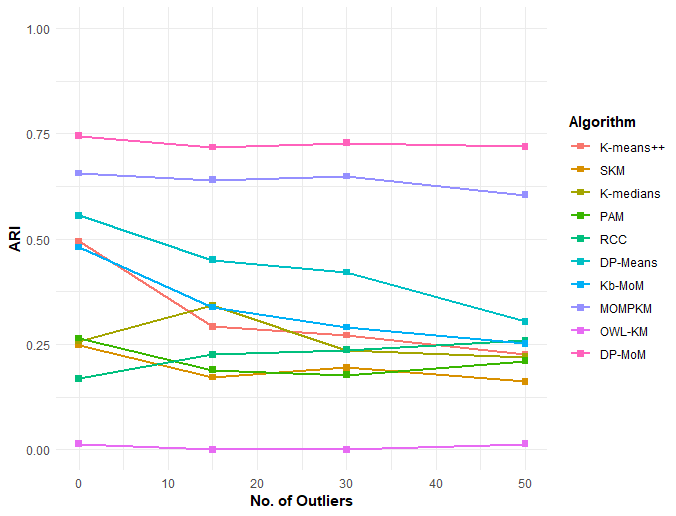
\includegraphics[width=0.4\textwidth]{Diagrams/plot-sim-ARI.png}
    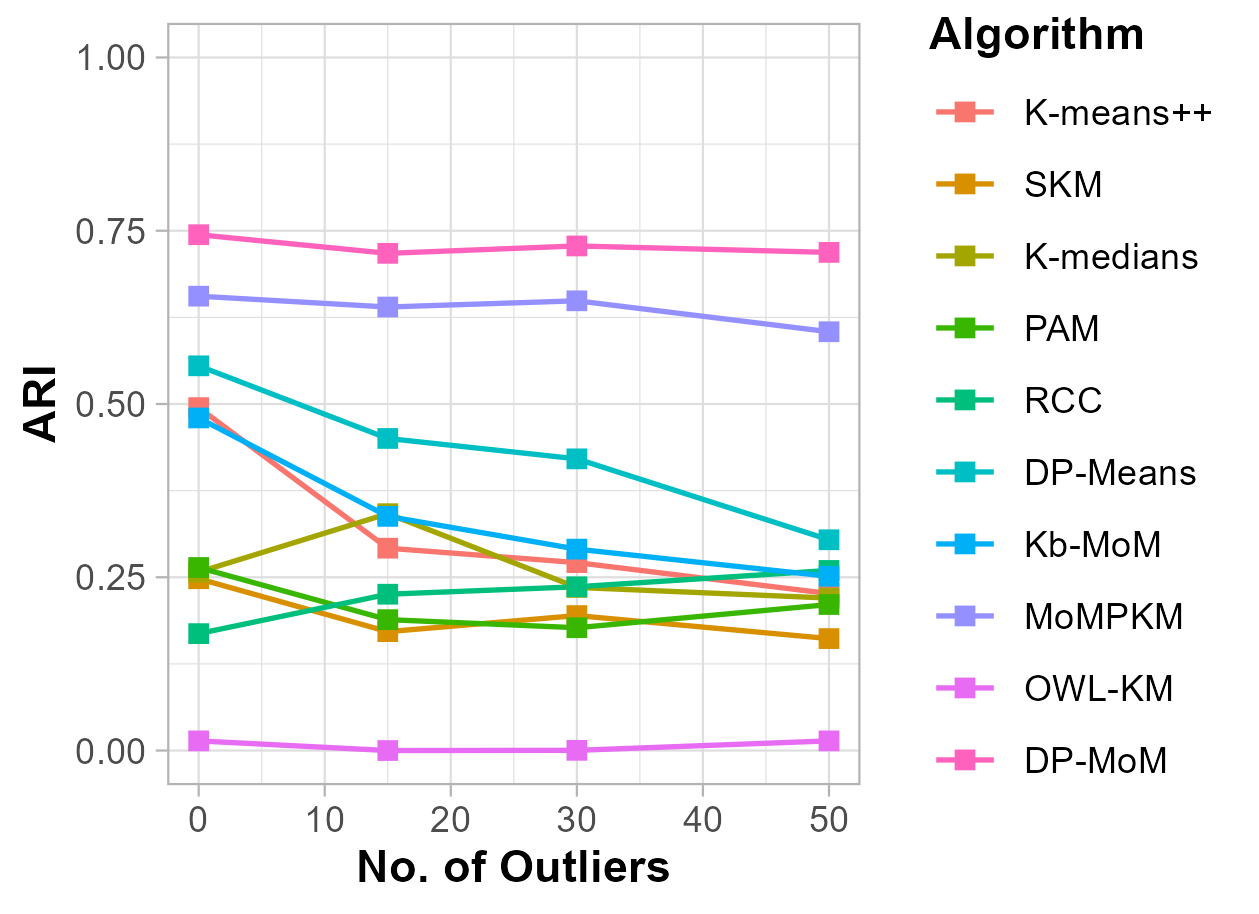
\includegraphics[width=0.38\textwidth]{Diagrams/plot-ari-sim-light-0.6.png}
    \caption{Line plots of ARI produced by different algorithms on simulated datasets, for increasingly higher number of outliers. DP-MoM performs uniformly better than all competing methods.}
    \label{fig:plot-sim-ari}
\end{figure}
\end{comment}

\subsubsection{Introducing Outliers - A Case Study}

We have picked the dataset \textit{Jain} \citep{jain-dataset} for this experiment. \textit{Jain} is a $2$-dimensional dataset with $373$ data points. The $2$ natural clusters are shaped like boomerangs, as can be seen in Figure 1 in Section \ref{sec:intro}. The performance of the algorithms was assessed on the original dataset. Afterward, several outliers were uniformly generated throughout the range of the data. $20$ fresh outliers were introduced in each of $4$ stages and at each stage, the algorithms were pitted against each other again. Even with the introduction of $80$ outliers, DP-MoM remained remarkably robust, consistently achieving a clustering accuracy of nearly $0.9$ in terms of ARI  (while the maximum ARI achieved was above that figure in all but one stage). Conversely, many other competing algorithms struggled to maintain their performance in the face of increasing outlier counts. 
% They exhibited significant fluctuations in ARI as the number of outliers rose. 
% Even the ones that maintained stability could only muster a measly ARI of $0.42$, as did all the other competing techniques.

\begin{comment}
\begin{figure}[!htb]
    \centering
    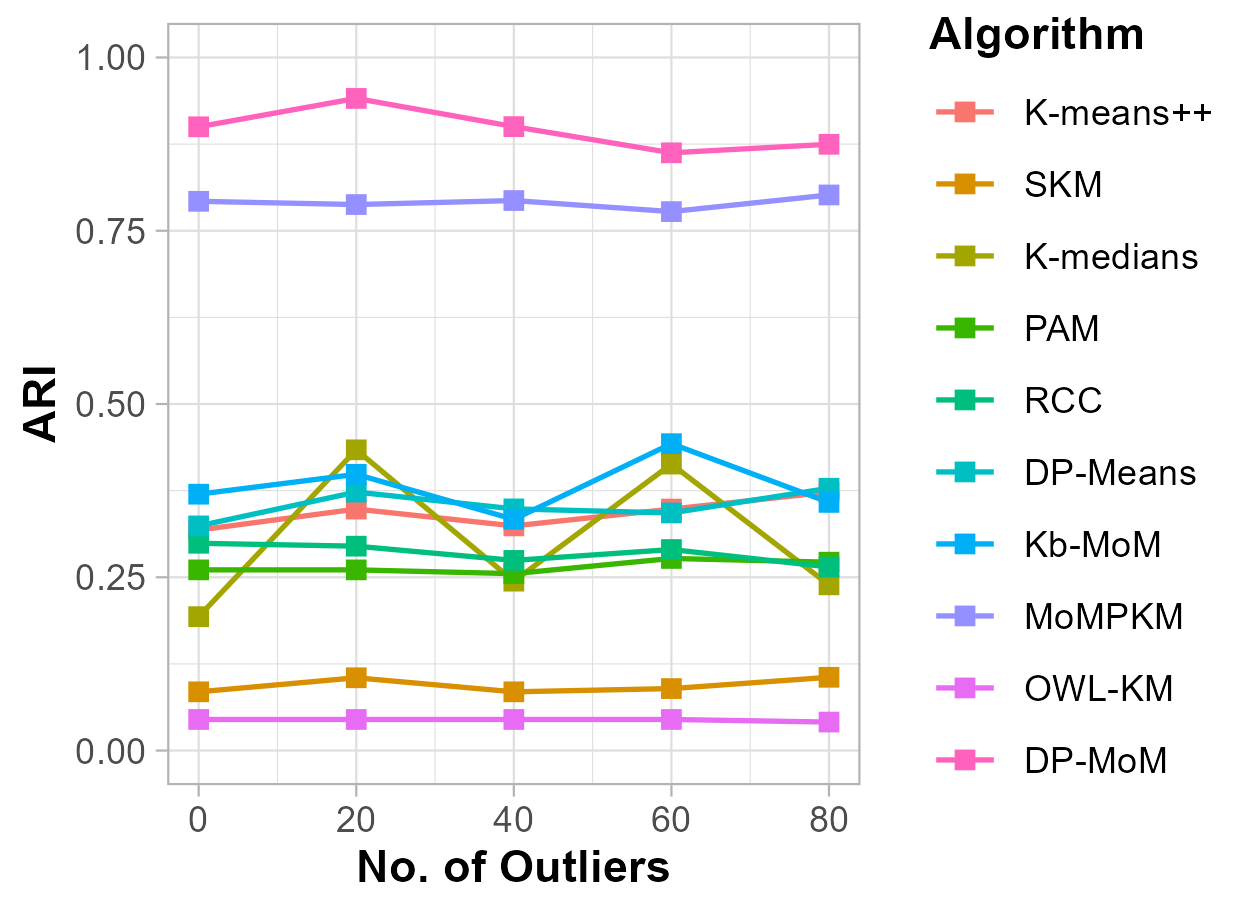
\includegraphics[width=0.38\textwidth]{Diagrams/plot-ari-jain-light-0.6.png}
    \caption{Line plots of ARI produced by different algorithms, for increasingly higher number of noisy observations introduced in the \textit{Jain} dataset. DP-MoM performs better than all competing methods.}
    \label{fig:plot-jain-ari}
\end{figure}
\end{comment}

\begin{figure}
\centering
\begin{minipage}{.46\textwidth}
  \centering
  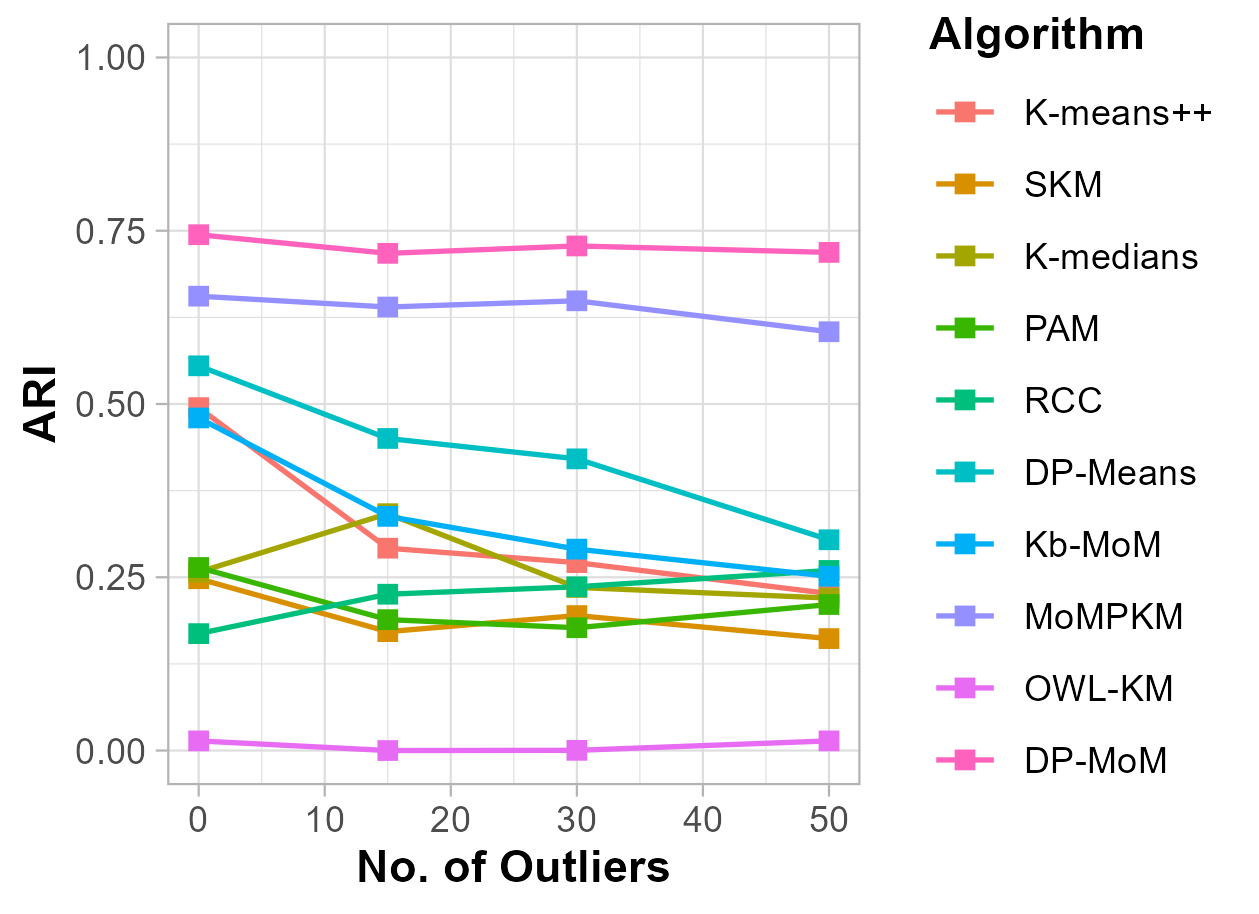
\includegraphics[width=.75\linewidth]{Diagrams/plot-ari-sim-light-0.6.png}
    \caption{Line plots of ARI produced by different algorithms on simulated datasets, for an increasingly higher number of outliers. DP-MoM performs uniformly better than all competing methods.}
    \label{fig:plot-sim-ari}
\end{minipage}%
\hspace{5mm}
\begin{minipage}{.46\textwidth}
  \centering
  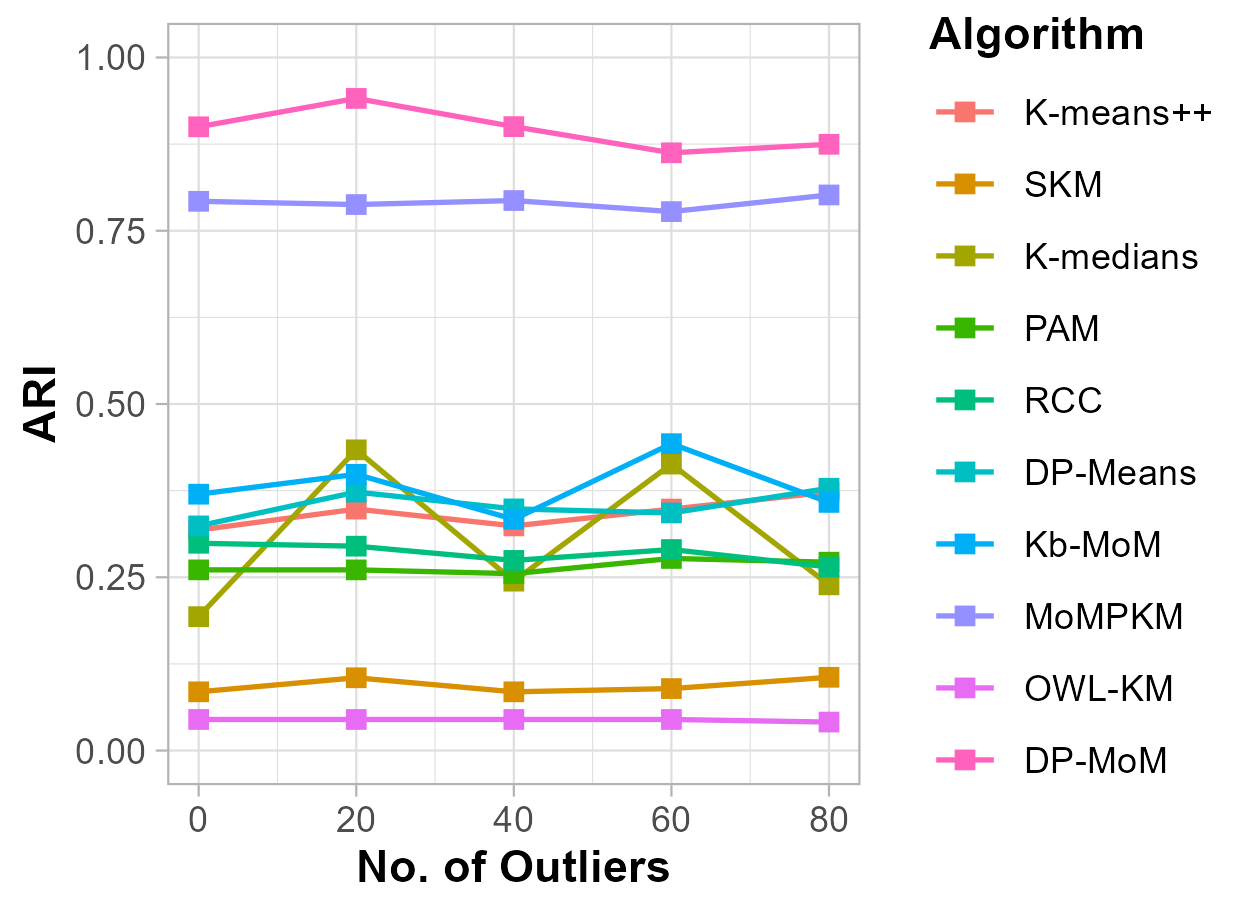
\includegraphics[width=.75\linewidth]{Diagrams/plot-ari-jain-light-0.6.png}
    \caption{Line plots of ARI produced by different algorithms for an increasingly higher number of noisy observations introduced in \textit{Jain} dataset. DP-MoM performs better than all competing methods.}
    \label{fig:plot-jain-ari}
\end{minipage}
\end{figure}

\subsection{Real Data Experiments}



% \subsubsection{Further Experiments}

For a comprehensive performance evaluation of our proposed clustering algorithm in situations where the underlying data distributions are unknown, we implement DP-MoM on several real datasets from the Compcancer database and the UCI Repository. Additionally, we implement some state-of-the-art clustering algorithms mentioned at the start of this section on the same datasets and compare the corresponding ARI values against that of DP-MoM. Since DP-MoM is a randomized algorithm in the sense that its cluster assignment is dependent on the initial dataset partitioning into buckets, we implement DP-MoM on each dataset $30$ times independently and report the median ARI. The same procedure is followed while reporting the ARI values for the competing algorithms.


\begin{table*}[!htb]
\renewcommand\theadfont{\bfseries}
\centering
\caption{Comparison of ARI for state-of-the-art algorithms vs. DP-MoM on Compcancer datasets}
% \vskip 1em
\resizebox{\linewidth}{!}{
\begin{tabular}{lccccccccccccc}
\toprule
\multirow[b]{2}{*}{\thead{\textbf{Dataset}}}
    &   \multicolumn{3}{c}{\thead{\textbf{Description}}}
        & \multicolumn{9}{c}{\thead{\textbf{State-of-the-Art Algorithms}}}
             & \multirow[b]{2}{*}{\thead{\textbf{DP-MoM}}}\\
\cmidrule(lr){2-4}\cmidrule(lr){5-13} %\cmidrule(lr){11-13}
% \toprule
% & $\mathbf{n}$ & $\mathbf{d}$ & $\mathbf{K}$ & \thead{KM++} & \thead{DPM} & \thead{KMed} & \thead{PAM} & \thead{K-bMoM} & \\
& \textit{\textbf{n}} & \textit{\textbf{p}} & \textit{\textbf{K}} & \thead{KM++} & \thead{SKM} & \thead{KMed} & \thead{PAM} & \thead{RCC} & \thead{DPM} & \thead{KbMoM} & \thead{MoMPKM} & \thead{OWL-KM}  & %\thead{DP-MoM}
\\
% \addlinespace
\midrule
\addlinespace
golub\_1999\_v2     & 72         & 1868                  & 3                  & 0.4334          & 0.6876    & 0.6116          & 0.7716    & 0.0000            & 0.6421         & 0.5664   & 0.6361       & 0.7438            & \textbf{0.7798} \\
west\_2001          & 49         & 1198                  & 2                  & 0.1527          & 0.0002    & 0.0886          & 0.1058    & 0.0000            & 0.1715         & 0.3061   & 0.4761       & \textbf{0.5613}   & 0.5035           \\
pomeroy\_2002\_v2   & 42         & 857                   & 5                  & 0.0000                  & 0.4924    & 0.0000                  & 0.0000            & 0.0000            & 0.0514         & 0.3583   & 0.4685       & 0.5175            & \textbf{0.5446} \\
singh\_2002         & 102        & 339                   & 2                  & 0.0259           & 0.0330   & 0.0259           & 0.0330    & 0.0000            & 0.0574         & 0.0330  & 0.3433       & 0.0483           & \textbf{0.8135} \\
tomlins\_v2         & 92         & 1288                  & 4                  & 0.1418          & 0.1245    & 0.0100          & 0.2134    & 0.0000            & 0.1814           & 0.1730   & 0.2775       & 0.1993            & \textbf{0.3985} \\
alizadeh\_2000\_v1  & 42         & 1095                  & 2                  & 0.0127          & 0 .0000           & 0.0000                  & 0.2564    & 0.0000            & 0.0023         & 0.0613   & 0.2714      & 0.0889             & \textbf{0.3716}  \\
armstrong\_2002\_v2 & 72         & 2194                  & 3                  & 0.5123          & 0.5448     & 0.6625          & 0.4584    & 0.0000            & 0.4660         & 0.4992   & 0.6365       & \textbf{0.9186} & 0.8332          \\
bredel\_2005        & 50         & 832                   & 3                  & 0.2000          & 0.3525    & 0.0098          & 0.4760    & 0.0000            & 0.0893         & 0.2315   & 0.4877       & 0.2996            & \textbf{0.5841}\\
\addlinespace
\midrule
Average Rank        &          &                    &                   & 7.2500          & 6.0000  & 7.7500 & 5.3125          & 9.6875    & 5.8750            & 5.7500         & 3.1250          &  3.0000           & \textbf{1.2500}\\
\bottomrule
\end{tabular}}
\label{table:compcancer}
\end{table*}


\begin{table*}[!htb]
\renewcommand\theadfont{\bfseries}
\centering
\caption{Comparison of ARI for state-of-the-art algorithms vs. DP-MoM on UCI datasets}
% \vskip 1em
\resizebox{\linewidth}{!}{
\begin{tabular}{lccccccccccccc}
\toprule
\multirow[b]{2}{*}{\thead{\textbf{Dataset}}}
    &   \multicolumn{3}{c}{\thead{\textbf{Description}}}
        & \multicolumn{9}{c}{\thead{\textbf{State-of-the-Art Algorithms}}}
             & \multirow[b]{2}{*}{\thead{\textbf{DP-MoM}}}\\
\cmidrule(lr){2-4}\cmidrule(lr){5-13} %\cmidrule(lr){11-13}
% \toprule
% & $\mathbf{n}$ & $\mathbf{d}$ & $\mathbf{K}$ & \thead{KM++} & \thead{DPM} & \thead{KMed} & \thead{PAM} & \thead{K-bMoM} & \\
& \textit{\textbf{n}} & \textit{\textbf{p}} & \textit{\textbf{K}} & \thead{KM++} & \thead{SKM} & \thead{KMed} & \thead{PAM} & \thead{RCC} & \thead{DPM} & \thead{KbMoM} & \thead{MoMPKM} & \thead{OWL-KM}  & %\thead{DP-MoM}
\\
% \addlinespace
\midrule
\addlinespace
Iris           & 150  & 4  & 3 & 0.7237 & 0.7960 & 0.7515 & 0.6325 & 0.8090 & 0.7515          & 0.7565 & 0.8647          & 0.6339  & \textbf{0.9799}  \\
Glass          & 214 & 9  & 7 & 0.3728 & 0.3595 & 0.3367 & 0.3501 & 0.3930 & \textbf{0.4472} & 0.3467 & 0.2484          & 0.2659 & 0.3190          \\
WDBC           & 569 & 30 & 2 & 0.4223 & 0.4223 & 0.4603 & 0.4587 & 0.4146 & 0.4479          & 0.4560 & \textbf{0.6839} & 0.5897 & 0.6798           \\
E.Coli         & 336 & 7  & 8 & 0.5001 & 0.4918 & 0.5346 & 0.5407 & 0.5350 & 0.6663          & 0.6216 & 0.4952          & 0.2174 & \textbf{0.7835} \\
Wine           & 178 & 13 & 3 & 0.4140 & 0.4287 & 0.4226 & 0.4189 & 0.3564 & 0.4094          & 0.4227 & 0.5518          & 0.3470 & \textbf{0.5820} \\
Thyroid        & 215 & 5  & 3 & 0.3936 & 0.2145 & 0.1450 & 0.2144 & 0.5186 & 0.4971          & 0.3032 & 0.5995          & 0.4392  & \textbf{0.8842} \\
Zoo            & 101 & 16 & 7 & 0.7376 & 0.7516 & 0.6730 & 0.6566 & 0.7173 & 0.8270          & 0.4978 & 0.7603          & 0.8408 & \textbf{0.8477} \\
soybean & 47 & 35 & 4 & 0.7143 & 0.7138 & 0.7108 & 0.7437 & 0.8268 & 0.7368          & 0.82678 & 0.7417          & 0.5452 & \textbf{0.9533} \\
\addlinespace
\midrule
Average Rank        &          &                    &                   & 6.5625          & 6.1875  & 6.9375 & 6.5000          & 5.1875    & 4.6875            & 5.4375         & 4.2500          &  7.2500           & \textbf{2.0000}\\
\bottomrule
\end{tabular}}
\label{table:uci}
\end{table*}


\subsubsection{Friedman's Rank Test} 
Friedman's rank test \citep{friedman} is employed to discern whether a significant difference exists in the performance of the algorithms applied to our datasets. This assessment unfolds across 3 stages. In stage $1$, the test encompasses all clustering algorithms under consideration. Moving to stage $2$, the analysis omits DP-MoM while incorporating the other algorithms. In stage $3$, both MoMPKM and DP-MoM are excluded from the test. The calculated p-values for these 3 stages are as follows: $1.57 \times 10^{-7}$, $0.0021$, and $0.0599$ respectively. The null hypothesis, which posits no significant variance in clustering accuracy among the tested algorithms, is rejected in the first and second stages, but accepted in the third stage. This outcome underscores that MoMPKM and DP-MoM emerge as the most proficient algorithms at our disposal. Further assessments indicate that MoMPKM is outperformed comprehensively by DP-MoM. 

\subsubsection{Sign Test and Wilcoxon Signed Rank (WSR) Test}

We also perform the \textit{Sign Test} and \textit{Wilcoxon Signed Rank Test} to compare our proposed algorithm individually with every other competing algorithm mentioned in Tables 1 and 2 and check whether DP-MoM performs significantly better than them. It is evident from the $p$-values that the null hypotheses: $H_{0s}:$ The said algorithm is better than DP-MoM (for \textit{Sign Test}) and $H_{0w}:$ The said algorithm is equivalent to our proposed framework DP-MoM (for \textit{WSR test}) are rejected in favor of the alternative $H_1:$ DP-MoM performs better than the other state-of-the-art algorithms in question for a test with level of significance $0.01$. In a majority of the cases, our proposed DP-MoM algorithm is the standout performer. However, in the 3 cases where its performance is suboptimal with respect to that of MoMPKM and OWL $k$-means, the results of the statistical tests presented in Table 3 of the Appendix, indicate that this drop in performance is not statistically significant at the specified level.

% Tables 4 and 5 in the Appendix provide the range of the penalty parameter $\lambda$ that enables us to cluster each dataset more efficiently. The predicted number of clusters are also displayed. Note that the number of clusters have been calculated after assigning the data points in the clusters containing less than $3$ observations, to the nearest cluster containing at least $3$ observations.

\begin{comment}
\begin{table}[!htb]
\renewcommand\theadfont{\bfseries}
\centering
\caption{Summary of the Statistical Test Results for level of significance $0.01$}
\vskip 0.7em
\resizebox{\linewidth}{!}{
\begin{tabular}{lccccccccccccc}
\toprule
\multirow[b]{2}{*}{\thead{\textbf{Clustering Algorithm}}}
    &   \multicolumn{2}{c}{\thead{\textbf{Sign Test}}}
        & \multicolumn{2}{c}{\thead{\textbf{WSR Test}}}
             \\
\cmidrule(lr){2-3}\cmidrule(lr){4-5} %\cmidrule(lr){11-13}
% \toprule
% & $\mathbf{n}$ & $\mathbf{d}$ & $\mathbf{K}$ & \thead{KM++} & \thead{DPM} & \thead{KMed} & \thead{PAM} & \thead{K-bMoM} & \\
& \thead{Statistic} & \thead{\textit{\textbf{p}}-value}  & \thead{Statistic} & \thead{\textit{\textbf{p}}-value} 
\\
% \addlinespace
\midrule
\addlinespace
$k$-means ++           & 15  & 0.0002594  & 135 & 0.0000305   \\
Sparse $k$-means          & 15  & 0.0002594  & 135 & 0.0000305          \\
$k$-medians           & 15  & 0.0002594  & 135 & 0.0000305         \\
Partition Around Medoids        & 15  & 0.0002594  & 134 & 0.0000458 \\
Robust Continuous Clustering           & 15  & 0.0002594  & 135 & 0.0000305 \\
DP means       & 15  & 0.0002594  & 133 & 0.0000763 \\
Kb MoM          & 15  & 0.0002594  & 135 & 0.0000305 \\
MoM Power $k$-means & 15  & 0.0002594  & 135 & 0.0000305 \\
OWL $k$-means & 14  & 0.0020900  & 125 & 0.0008392\\
\addlinespace
\bottomrule
\end{tabular}
}
\label{table:statistical tests}
\end{table}
\end{comment}


\begin{comment}
\begin{table}[!htb]
\renewcommand\theadfont{\bfseries}
\centering
\caption{Range of optimal $\lambda$ and estimated number of clusters for implementing DP-MoM on UCI datasets}
\vskip 1em
\resizebox{\linewidth}{!}{
\begin{tabular}{lcc}
\toprule
{\thead{\textbf{Dataset}}}
    &   \multicolumn{1}{c}{\thead{\textbf{Range of Optimal $\lambda$}}}
        & \multicolumn{1}{c}{{\textbf{Estimated Clusters}}}\\
% \addlinespace
\midrule
\addlinespace
Iris          & 5.129 - 6.535  & 3 \\
Glass         & 4.207 - 18.841  &  6 \\
WDBC           & 2.5$\times 10^6$ - 6$\times 10^6$  & 2 \\
E. Coli       & 0.3008 - 0.3571  & 8 \\
Wine         &  3.78$\times 10^5$ - 3.93$\times 10^5$ & 2 \\
Thyroid       & 1769 - 2123  & 5 \\
Zoo          & 7.048 - 10.360  & 6 \\
soybean & 18.59 - 25.70  & 4 \\
\addlinespace
\bottomrule
\end{tabular}
}
\label{table:lambda-uci}
\end{table}


\begin{table}[!htb]
\renewcommand\theadfont{\bfseries}
\centering
\caption{Range of optimal $\lambda$ and estimated number of clusters for implementing DP-MoM on Compcancer datasets}
\vskip 1em
\resizebox{\linewidth}{!}{
\begin{tabular}{lcc}
\toprule
{\thead{\textbf{Dataset}}}
    &   \multicolumn{1}{c}{\thead{\textbf{Range of Optimal $\lambda$}}}
        & \multicolumn{1}{c}{\thead{\textbf{Estimated Clusters}}}\\
% \addlinespace
\midrule
\addlinespace
golub\_1999\_v2          & 2.48$\times 10^9$ - 3.05$\times 10^9$ & 3   \\
west\_2001         & 1.77$\times 10^9$  - 3.11$\times 10^9$ &  2         \\
pomeroy\_2002\_v2           & 2.94$\times 10^9$ - 4.70$\times 10^9$ & 4         \\
singh\_2002       & 0.14$\times 10^9$ - 0.17$\times 10^9$ & 2 \\
tomlins\_v2         &  175.6 - 308.0 & 2 \\
alizadeh\_2000\_v1       & 762.8 - 780.0  & 2 \\
armstrong\_2002\_v2          & 5.85$\times 10^9$ - 7.08$\times 10^9$ & 3 \\
bredel\_2005 & 672.4 - 978.8  & 2 \\
\addlinespace
\bottomrule
\end{tabular}
}
\label{table:lambda-compcancer}
\end{table}
\end{comment}

\section{Discussion}

In this article, we proposed a new clustering algorithm that tactfully integrates two major clustering paradigms, viz., centroid-based clustering and model-based clustering that is intended to perform well on noisy or outlier-infested data. We utilize the Median-of-Means (MoM) estimator to deal with noise or outliers present in data, and Bayesian nonparametric modeling ensures that the number of clusters need not be specified earlier. Unlike conventional clustering algorithms, which typically tackle only one of these challenges, our proposed algorithm adeptly tackles both at the same time. Following our comprehensive theoretical analysis of error rate bounds, augmented by extensive simulation studies and real-world data analysis, we showcase the superiority of our methods against some of the most prominent clustering techniques. 

%\section*{References}

\bibliographystyle{apalike}
\bibliography{references}


%%%%%%%%%%%%%%%%%%%%%%%%%%%%%%%%%%%%%%%%%%%%%%%%%%%%%%%%%%%%

\appendix


% \begin{center}
%     \LARGE{\bfseries Supplementary Material to ``Robust and Automatic Data Clustering:\\ Dirichlet Process meets Median-of-Means"}
% \end{center}
% \vspace{1cm}

% \section{Introduction}

\section{An Additional Lemma}

\begin{lemma}\label{lemma-bound-Psi}
    For all $\bm{x}\in [-M,M]^p$ and $\bm{\Theta}\in \mathscr{G}$, \[0\le \Psi(d(\bm{x},\bm{\theta}_1), d(\bm{x},\bm{\theta}_2),\cdots, d(\bm{x},\bm{\theta}_K) )\le 4M^2p.\]
    Consequently, $\sup_{f\in \mathcal{F}}\|f\|_{\infty}\le 4M^2p$. 
\end{lemma}

\begin{proof}
%     From the non-negativity of $\Psi(.)$, we get that $\Psi(d(\bm{x},\bm{\theta}_1), d(\bm{x},\bm{\theta}_2),\cdots, d(\bm{x},\bm{\theta}_K) )\ge 0$ for every $x\in [-M,M]^p$ and $\bm{\Theta}\in [-M,M]^{k\times p}$. Now,\begin{align*}
%         &\Psi(d(\bm{x},\bm{\theta}_1), d(\bm{x},\bm{\theta}_2),\cdots, d(\bm{x},\bm{\theta}_K) )\\
%         &=\min_{1\le j\le K}\|\bm{x}-\bm{\theta}_j\|_2^2\\
%         & \le \max_{1\le j\le K}\|\bm{x}-\bm{\theta}_j\|_2^2\\
%         & \le 4M^2p
%     \end{align*}
    Firstly,
    \begin{equation*}
        \Psi(d(\bm{x},\bm{\theta}_1), d(\bm{x},\bm{\theta}_2),\cdots, d(\bm{x},\bm{\theta}_K) ) = \min_{1\le j\le K}\|\bm{x}-\bm{\theta}_j\|_2^2 \le \max_{1\le j\le K}\|\bm{x}-\bm{\theta}_j\|_2^2 \le 4M^2p.
    \end{equation*}

    Since $\bm{x}$ is arbitrary, the second part of the lemma follows immediately.
\end{proof}

\section{Proofs of Results from Section \ref{sec:theory}}


\subsection{Proof of Theorem \ref{thm-2-diff-Pn-P}}

\begin{proof}
    From Lemma \ref{lemma-bound-Psi}, we see that $\sup_{f\in \mathcal{F}}\|f\|_{\infty}\le 4M^2p$. Thanks to Theorem 4.10 of \citep{wainwright_2019}, for any $\delta \in (0,1)$, with probability at least $1-\delta$, 
    \begin{align*}
        \sup_{f\in \mathcal{F}}|P_n f-Pf| &\le 2\cdot\mathcal{R}_n(\mathcal{F})+\sup_{f\in \mathcal{F}}\|f\|_{\infty}\sqrt{\frac{2\log(2/\delta)}{n}}\\
        &\le 96\sqrt{\pi}M^2(Kp)^{3/2}n^{-1/2}+4\sqrt{2}M^2p\log^{\tfrac{1}{2}}\left(\frac{2}{\delta}\right) n^{-1/2}.
    \end{align*}
\end{proof}


\subsection{Proof of Theorem \ref{thm-4-MoM}}

\begin{proof} 
We represent the empirical distribution of $\{\bX_i\}_{i \in B_\ell}$ by $P_{B_{\ell}}$. Fix $\epsilon>0$. We will first establish a concentration inequality on $\sup_{\bTheta \in \mathscr{G}} |\text{MoM}_L^n (f_{\bTheta}) - P f_{\bTheta} |$. To that end, we bound the probabilities of the events $\{\sup_{\bTheta \in \mathscr{G}}(\text{MoM}_L^n (f_{\bTheta}) - P f_{\bTheta}) >\epsilon\}$ and $\{\sup_{\bTheta \in \mathscr{G}}  ( P f_{\bTheta} - \text{MoM}_L^n (f_{\bTheta})) > \epsilon\}$ individually. Note that 
\begin{equation}
\sup_{\bTheta \in \mathscr{G}}\sum_{\ell = 1}^L \one\left\{(P-P_{B_\ell})f_{\bTheta} > \epsilon\right\} > \frac{L}{2} \implies \sup_{\bTheta \in \mathscr{G}} (P f_{\bTheta} - \text{MoM}_L^n (f_{\bTheta})) > \epsilon.
\end{equation}
To see this, suppose on the contrary that \[\sup_{\bTheta \in \mathscr{G}}  (P f_{\bTheta} - \text{MoM}_L^n (f_{\bTheta})) \le \epsilon\] but \[\sup_{\bTheta \in \mathscr{G}}\sum_{\ell = 1}^L \one\left\{(P-P_{B_\ell})f_{\bTheta} > \epsilon\right\} > \frac{L}{2}\]. 
Then for all $\bm{\Theta}\in \mathscr{G}$, we must have \[\sup_{\bTheta \in \mathscr{G}}\sum_{\ell = 1}^L \one\left\{(P-P_{B_\ell})f_{\bTheta} > \epsilon\right\} > \frac{L}{2}\] which implies that for all $\bm{\Theta}\in \mathscr{G}$ \[\sum_{\ell = 1}^L \one\left\{(P-P_{B_\ell})f_{\bTheta} \le \epsilon\right\} \ge \frac{L}{2} \implies \sum_{\ell = 1}^L \one\left\{(P-P_{B_\ell})f_{\bTheta} > \epsilon\right\} \le \frac{L}{2}\] which in turn implies that \[\sup_{\bTheta \in \mathscr{G}}\sum_{\ell = 1}^L \one\left\{(P-P_{B_\ell})f_{\bTheta} > \epsilon\right\} \le \frac{L}{2}\] which is a contradiction. Let $\varphi(t) = (t-1) \one\{1 \le t \le 2\} + \one\{t >2\}$ where $\one\{\cdot\}$ is the indicator function. Evidently,
\begin{equation}
    \label{eq6}
    \one\{t \ge 2\} \le \varphi(t) \le \one\{t \ge 1\}.
\end{equation} 
We observe that
\begingroup
\allowdisplaybreaks
\begin{align}
    \sup_{\bTheta \in \mathscr{G}}\sum_{\ell = 1}^L \one\left\{(P-P_{B_\ell})f_{\bTheta} > \epsilon\right\}
    % \le & \sup_{\bTheta \in \mathscr{G}}\sum_{\ell \in \cL} \one\left\{(P-P_{B_\ell})f_{\bTheta} > \epsilon\right\} + |\cO|\nonumber\\
    % \le & \sup_{\bTheta \in \mathscr{G}}\sum_{\ell \in \cL}  \varphi\left(\frac{2(P-P_{B_\ell})f_{\bTheta}}{\epsilon}\right) + |\cO|\nonumber\\
    & \le \sup_{\bTheta \in \mathscr{G}}\sum_{\ell \in \cL}  \E \varphi\left(\frac{2(P-P_{B_\ell})f_{\bTheta}}{\epsilon}\right)  + |\cO|\nonumber\\
    & ~+\sup_{\bTheta \in \mathscr{G}}\sum_{\ell \in \cL}  \bigg[ \varphi\left(\frac{2(P-P_{B_\ell})f_{\bTheta}}{\epsilon}\right)   - \E \varphi\left(\frac{2(P-P_{B_\ell})f_{\bTheta}}{\epsilon}\right)\bigg]. \label{eq01}
\end{align}
\endgroup
Towards bounding $\sup_{\bTheta \in \mathscr{G}}\sum_{\ell = 1}^L \one\left\{(P-P_{B_\ell})f_{\bTheta} > \epsilon\right\}$, we first bound $\E \varphi\left(\frac{2(P-P_{B_\ell})f_{\bTheta}}{\epsilon}\right)$. Note that
\begingroup
\allowdisplaybreaks
% \begin{align}
% \small 
%   \E \varphi\left(\frac{2(P-P_{B_\ell})f_{\bTheta}}{\epsilon}\right) 
%   \le  \E \left[ \one\left\{\frac{2(P-P_{B_\ell})f_{\bTheta}}{\epsilon} > 1 \right\}\right] \nonumber  = & \sP \left[ (P-P_{B_\ell})f_{\bTheta}>\frac{\epsilon}{2} \right] \nonumber \\ 
%   \le & \exp\left\{-\frac{b \epsilon^2}{32 M^4 K^2 p^2}\right\}
% \end{align} 
\begin{equation*}
    \E \varphi\left(\frac{2(P-P_{B_\ell})f_{\bTheta}}{\epsilon}\right) \le  %\E \left[ \one\left\{\frac{2(P-P_{B_\ell})f_{\bTheta}}{\epsilon} > 1 \right\}\right] = 
    \sP \left[ (P-P_{B_\ell})f_{\bTheta}>\frac{\epsilon}{2} \right] \le \exp\left\{-\frac{b \epsilon^2}{32 M^4 K^2 p^2}\right\}.
\end{equation*}

The last inequality follows by Hoeffding's inequality after observing that $\displaystyle \mathbb{E} P_{B_{\ell}}f_{\bm{\Theta}}=Pf_{\bm{\Theta}}$ and by Lemma \ref{lemma-bound-Psi}.
\endgroup
 We now turn to bounding the term \[ \sup_{\bTheta \in \mathscr{G}}\sum_{\ell \in \cL}  \bigg[ \varphi\left(\frac{2(P-P_{B_\ell})f_{\bTheta}}{\epsilon}\right)   - \E \varphi\left(\frac{2(P-P_{B_\ell})f_{\bTheta}}{\epsilon}\right)\bigg]. \] Appealing to Theorem 26.5 of \citep{shalev-shwartz_ben-david_2014}, for all $ \bTheta \in \mathscr{G}$, we have
\begin{align}
  &\frac{1}{L}\sum_{\ell \in \cL}   \varphi\left(\frac{2(P-P_{B_\ell})f_{\bTheta}}{\epsilon}\right)- \E \left[\frac{1}{L}\sum_{\ell \in \cL}  \varphi\left(\frac{2(P-P_{B_\ell})f_{\bTheta}}{\epsilon}\right) \right]\nonumber \\
  &\le 2\E\left[\sup_{\bTheta \in \mathscr{G}}\frac{1}{L}\sum_{\ell \in \cL}\sigma_\ell  \varphi\left(\frac{2(P-P_{B_\ell})f_{\bTheta}}{\epsilon}\right) \right] + \delta.  \label{eq5}
\end{align}
with probability at least $1-2e^{-L\delta^2/2}$,
where $\{\sigma_\ell\}_{\ell \in \mathcal{L}}$ are i.i.d. Rademacher random variables independent of the sample $\mathcal{X}$. Consider i.i.d. Rademacher random variables $\{\xi_i\}_{i=1}^n$ independent of  $\{\sigma_\ell\}_{\ell \in \mathcal{L}}$. As a consequence of equation \eqref{eq5}, we get,  
\begingroup
\allowdisplaybreaks
\begin{align}
     & \frac{1}{L}\sup_{\bTheta \in \mathscr{G}}\sum_{\ell \in \cL}  \bigg[ \varphi\left(\frac{2(P-P_{B_\ell})f_{\bTheta}}{\epsilon}\right)  - \E \varphi\left(\frac{2(P-P_{B_\ell})f_{\bTheta}}{\epsilon}\right)\bigg] \nonumber\\
     & \le \frac{4}{L \epsilon}\E\left[\sup_{\bTheta \in \mathscr{G}}\sum_{\ell \in \cL}\sigma_\ell  (P-P_{B_\ell})f_{\bTheta} \right]+ \delta. \label{eq7} 
     \end{align}
     Equation \eqref{eq7} follows from the fact that $\varphi(\cdot)$ is 1-Lipschitz and Lemma 26.9 of \citep{shalev-shwartz_ben-david_2014}. We now consider random variables $\mathcal{X}^\prime=\{\bX_1^\prime, \dots, \bX_n^\prime\}$, which are i.i.d. and follow the law $P$. Equation \eqref{eq7} further yields
     \begin{align}
     = & \frac{4}{L \epsilon}\E\left[\sup_{\bTheta \in \mathscr{G}}\sum_{\ell \in \cL}\sigma_\ell  \E_{\mathcal{X}^\prime}\left((P^\prime_{B_\ell}-P_{B_\ell})f_{\bTheta}\right) \right]+ \delta \nonumber \\
     \le & \frac{4}{L \epsilon}\E\left[\sup_{\bTheta \in \mathscr{G}}\sum_{\ell \in \cL}\sigma_\ell  (P^\prime_{B_\ell}-P_{B_\ell})f_{\bTheta} \right]+ \delta \label{rad-comp} \\
     = & \frac{4}{L \epsilon}\E\left[\sup_{\bTheta \in \mathscr{G}}\sum_{\ell \in \cL}\sigma_\ell  \frac{1}{b}\sum_{i \in B_\ell}(f_{\bTheta}(\bX_i^\prime)-f_{\bTheta}(\bX_i)) \right]+ \delta \nonumber \\
     = & \frac{4}{b L \epsilon}\E\left[\sup_{\bTheta \in \mathscr{G}}\sum_{\ell \in \cL}\sigma_\ell  \sum_{i \in B_\ell} \xi_i(f_{\bTheta}(\bX_i^\prime)-f_{\bTheta}(\bX_i)) \right]+ \delta \label{eq8} \\
     = & \frac{4}{n \epsilon}\E\left[\sup_{\bTheta \in \mathscr{G}}\sum_{\ell \in \cL}  \sum_{i \in B_\ell} \sigma_\ell \xi_i(f_{\bTheta}(\bX_i^\prime)-f_{\bTheta}(\bX_i)) \right]+ \delta \nonumber \\
     = & \frac{4}{n \epsilon}\E\left[\sup_{\bTheta \in \mathscr{G}} \sum_{i \in \J} \gamma_i (f_{\bTheta}(\bX_i^\prime)-f_{\bTheta}(\bX_i)) \right]+ \delta \label{eq9} \\
     \le &  \frac{4}{n \epsilon}\E\left[\sup_{\bTheta \in \mathscr{G}} \sum_{i \in \J} \gamma_i f_{\bTheta}(\bX_i^\prime)+ \sup_{\bTheta \in \mathscr{G}} \sum_{i \in \J} \gamma_i f_{\bTheta}(\bX_i) \right]+ \delta\\
     \le & \frac{4}{n \epsilon}\E\left[\sup_{\bTheta \in \mathscr{G}} \sum_{i \in \J} \gamma_i f_{\bTheta}(\bX_i^\prime)\right]+\E\left[ \sup_{\bTheta \in \mathscr{G}} \sum_{i \in \J} \gamma_i f_{\bTheta}(\bX_i) \right]+ \delta\\
     = & \frac{8}{n \epsilon}\E\left[\sup_{\bTheta \in \mathscr{G}} \sum_{i \in \J} \gamma_i f_{\bTheta}(\bX_i) \right]+ \delta \nonumber \\
     \le & \frac{8}{n \epsilon} 48 \sqrt{\pi}  M^2  (Kp)^{3/2}  \sqrt{|\J|} + \delta \label{eq10} \\
     \le & \frac{384}{n \epsilon}  \sqrt{\pi}  M^2  (Kp)^{3/2} \sqrt{|\I|} + \delta. \label{eq11}
\end{align}
\endgroup
The inequality \eqref{rad-comp} follows by employing Jensen's inequality as supremum is a convex function, and the expectation in the second step is taken with respect to both the original sample $\mathcal{X}$ as well as the ghost sample $\mathcal{X}'$ and the Rademacher random variables $\{\sigma_{\ell}\}_{\ell\ge 1}$.
Here $\J$ is the set of observations in the partitions not containing an outlier. Equation \eqref{eq8} follows from the fact that $$(f_{\bTheta}(\bX_i^\prime)-f_{\bTheta}(\bX_i)) \overset{d}{=\joinrel=} \xi_i(f_{\bTheta}(\bX_i^\prime)-f_{\bTheta}(\bX_i))$$ as $\{\xi_i\}_{i\ge 1}$ are Rademacher random variables independent of the sample $\mathcal{X}$. In equation \eqref{eq9}, $\{\gamma_i\}_{i \in \mathcal{J}}$ are independent Rademacher random variables since the product of 2 independent Rademacher random variables is also a Rademacher random variable. Equation \eqref{eq10} follows by Theorem \ref{thm-1-RnF}.
Thus, combining equations \eqref{eq5}, \eqref{eq7}, and \eqref{eq11}, we conclude that,  with probability of at least $1-2e^{-L \delta^2/2}$, 
\begin{equation}
    \sup_{\bTheta \in \mathscr{G}}\sum_{\ell = 1}^L \one\left\{(P-P_{B_\ell})f_{\bTheta} > \epsilon\right\} \le  L \left( \exp\left\{-\frac{b \epsilon^2}{32  M^4 K^2 p^2}\right\}+ \frac{|\cO|}{L} + \frac{384}{n \epsilon}  \sqrt{\pi} M^2  (Kp)^{3/2} \sqrt{|\I|} + \delta\right). \label{eq12}
\end{equation}
We choose $\delta = \frac{2}{4+\eta} - \frac{|\cO|}{L}$, and $$\epsilon = \max\left\{\sqrt{32  M^4 \log\left(\frac{4(\eta+4)}{\eta}\right)}KpL^{1/2}n^{-1/2}, \frac{1536(\eta+4)  M^2 \sqrt{\pi}}{\eta} (Kp)^{3/2} |\I|^{1/2}n^{-1}\right\}.$$ This makes the right-hand side of \eqref{eq12} strictly smaller than $\frac{L}{2}$.
% In the unusual situation where you want a paper to appear in the
% references without citing it in the main text, use \nocite
%\nocite{langley00}
Thus, we have shown that 
\begin{align*}
     \sP\left( \sup_{\bTheta \in \mathscr{G}} (Pf_{\bTheta} - \text{MoM}^n_L (f_{\bTheta}))> \epsilon \right) \le 2e^{-L \delta^2/2}.
 \end{align*}
% \begin{align*}
%     &P\left( \sup_{\bTheta \in \mathscr{G}} (Pf_{\bTheta} - \text{MoM}^n_L (f_{\bTheta}))> \epsilon \right) \\
%     & \le P\left(\sup_{\bTheta \in \mathscr{G}}\sum_{\ell = 1}^L \one\left\{(P-P_{B_\ell})f_{\bTheta} > \epsilon\right\} \ge L/2\right) \le e^{-2L \delta^2}.
% \end{align*}
By a similar argument, it follows that,
\begin{align*}
    \sP\left( \sup_{\bTheta \in \mathscr{G}} (\text{MoM}^n_L (f_{\bTheta}) -Pf_{\bTheta} ) > \epsilon \right) \le 2e^{-L \delta^2/2}.
\end{align*}
From the aforementioned inequalities, we obtain, 
\[\sP\left( \sup_{\bTheta \in \mathscr{G}} |\text{MoM}^n_L (f_{\bTheta}) -Pf_{\bTheta} | > \epsilon \right) \le 4e^{-L \delta^2/2}.\]
i.e., with at least probability $1-4e^{-L \delta^2/2}$,
\begin{align*}
    & \sup_{\bTheta \in \mathscr{G}} |\text{MoM}^n_L (f_{\bTheta}) -Pf_{\bTheta} | \\
    &\le \max\left\{\sqrt{32  M^4 \log\left(\frac{4(\eta+4)}{\eta}\right)}KpL^{1/2}n^{-1/2}, \frac{1536(\eta+4)  M^2 \sqrt{\pi}}{\eta} (Kp)^{3/2} |\I|^{1/2}n^{-1}\right\}\\
    &\lesssim \max\left\{ KpL^{1/2}n^{-1/2}, (Kp)^{3/2}  |\I|^{1/2}n^{-1}\right\}.
\end{align*}
\end{proof}


\section{Machine Specifications}

All the simulation as well real data experiments were conducted using a computer equipped with Intel(R) Core(TM)i3-7020U 2.30GHz  processor, 4GB RAM, 64-bit Windows 10 operating  system in the \texttt{R} programming language \citep{R-lang}.


\section{Parameter Selection}
The tuning parameter $\epsilon$ is set to 1. The learning rate $\eta$ is typically chosen to be the power of 10 which is of the order of the square of the maximum pairwise distance in the dataset, or one lower than that i.e. if the maximum squared separation between any two observations in the data is $D$, then we set $\eta = 10 ^{\lceil 2\log_{10} D \rceil /2}$ or $10^{\lceil 2\log_{10} D \rceil /2-1}$ depending on which of these values aids efficient clustering using our proposed method, where $\lceil \cdot \rceil$ represents the ceiling function. Our proposed framework enables us to automatically detect the appropriate number of clusters based on the value of the penalty parameter $\lambda$ which is optimized by grid-searching.

The first step in our proposed algorithm is partitioning the dataset randomly. This is achieved by choosing a uniform permutation of the data points and then placing them in different buckets in the order of the permutation. Though this technique achieves randomness in terms of partitioning the data, arbitrary partitioning may lead to undesirable results, which is why the partitioning (or permutation, for that matter) needs to be carefully chosen. We resort to a form of grid search to solve this problem. We determine $\lambda_{\min}$ and $\lambda_{\max}$, respectively, the minimum and maximum pairwise squared distance between the data points. $11$ equally-spaced points $\lambda_{\min} =\lambda^1_1<\lambda^1_2< \cdots < \lambda^1_{10}<\lambda^1_{11}=\lambda_{\max}$ are picked, and the algorithm is run for these values and for all values of number of partitions, $L$, such that $2<L<\frac{n}{3}$. We select $\lambda^1_{i^*}$ corresponding to the most accurate clustering and divide its neighborhood $[\lambda^1_{i^*-1},\lambda_{i^*-1}]$  $\left([\lambda^1_1,\lambda^1_2]\operatorname{ or }[\lambda^1_{10}, \lambda^1_{11}]\right)$ into $20$ divisions and re-run the algorithm as we did in the interval $[\lambda_{\min}, \lambda_{\max}]$. We repeat this again so that the feasible range for the penalty parameter $\lambda$ has been segmented to the order of $10^3$. We obtain the permutation corresponding to the most accurate clustering in the three stages above and use this particular permutation to partition the data for further experiments.

We imitate the above experiment, except that this time, we use the permutation of the data points obtained from the said grid-searching to partition the data. We then choose the $\lambda$ and $L$ values for which the best clustering accuracy is attained. We call them $\lambda_{opt}$ and $L_{opt}$. Since our proposed algorithm is a randomized one, we cannot readily conclude that $\lambda_{opt}$ and $L_{opt}$ are the only values corresponding to which we will obtain high clustering accuracy. In fact, for another repetition of the above experiment, we may not obtain an identical favorable permutation or the same optimal $\lambda$ and $L$ values. So, we repeat the aforementioned grid-searching experiment a number of times (say about 30 times) so that we may obtain a range of $\lambda$ and a range of $L$ that will be suitable to work with to derive the best results out of the proposed framework. We choose the median of the clustering accuracies, measured with the Adjusted Rand Index (ARI) \citep{Hubert1985} so obtained, as a representative of the clustering accuracy of the algorithm.

We may limit our grid search to the values of $L$ that are of the order of $n$, i.e., $L\asymp n$. This is because the breakdown point of the MoM estimator is $\left[(L-1)/2\right]/n$ \citep{rodriguez2019breakdown}. Hence, choosing very small values of $L$, i.e., $L=o(n)$, will severely affect the quality of clustering in the presence of outliers. Assumption \ref{ass-5-L} which requires the number of outliers $|\mathcal{O}|$ to be less than half the number of partitions, therefore implies that the MoM estimator and consequently the centroid estimates do not break down in the presence of outlying observations. 


\section{Additional Tables}

Table 3 provides the $p$-values and test statistic values for the sign test and the Wilcoxon Signed Rank test conducted to determine whether DP-MoM performs significantly better than other state-of-the-art clustering techniques in terms of the ARI.

\begin{table}[!htb]
\renewcommand\theadfont{\bfseries}
\centering
\caption{Summary of the Statistical Test Results for level of significance $0.01$}
\vskip 0.7em
\resizebox{0.54\linewidth}{!}{
\begin{tabular}{lccccccccccccc}
\toprule
\multirow[b]{2}{*}{\thead{\textbf{Clustering Algorithm}}}
    &   \multicolumn{2}{c}{\thead{\textbf{Sign Test}}}
        & \multicolumn{2}{c}{\thead{\textbf{WSR Test}}}
             \\
\cmidrule(lr){2-3}\cmidrule(lr){4-5} %\cmidrule(lr){11-13}
% \toprule
% & $\mathbf{n}$ & $\mathbf{d}$ & $\mathbf{K}$ & \thead{KM++} & \thead{DPM} & \thead{KMed} & \thead{PAM} & \thead{K-bMoM} & \\
& \thead{Statistic} & \thead{\textit{\textbf{p}}-value}  & \thead{Statistic} & \thead{\textit{\textbf{p}}-value} 
\\
% \addlinespace
\midrule
\addlinespace
$k$-means ++           & 15  & 0.0002594  & 135 & 0.0000305   \\
Sparse $k$-means          & 15  & 0.0002594  & 135 & 0.0000305          \\
$k$-medians           & 15  & 0.0002594  & 135 & 0.0000305         \\
Partition Around Medoids        & 15  & 0.0002594  & 134 & 0.0000458 \\
Robust Continuous Clustering           & 15  & 0.0002594  & 135 & 0.0000305 \\
DP means       & 15  & 0.0002594  & 133 & 0.0000763 \\
Kb MoM          & 15  & 0.0002594  & 135 & 0.0000305 \\
MoM Power $k$-means & 15  & 0.0002594  & 135 & 0.0000305 \\
OWL $k$-means & 14  & 0.0020900  & 125 & 0.0008392\\
\addlinespace
\bottomrule
\end{tabular}
}
\label{table:statistical tests}
\end{table}

Tables 4 and 5 below provide the range of the penalty parameter $\lambda$ that enables us to cluster each dataset more efficiently. The predicted number of clusters is also presented. Note that the number of clusters has been calculated after assigning the data points in the clusters containing less than $3$ observations to the nearest cluster containing at least $3$ observations. 

\begin{table}[!htb]
\renewcommand\theadfont{\bfseries}
\centering
\caption{Range of optimal $\lambda$ and estimated number of clusters for implementing DP-MoM on UCI datasets}
\vskip 1em
\resizebox{0.4\linewidth}{!}{
\begin{tabular}{lcc}
\toprule
{\thead{\textbf{Dataset}}}
    &   \multicolumn{1}{c}{\thead{\textbf{Range of Optimal $\lambda$}}}
        & \multicolumn{1}{c}{{\textbf{Estimated Clusters}}}\\
% \addlinespace
\midrule
\addlinespace
Iris          & 5.129 - 6.535  & 3 \\
Glass         & 4.207 - 18.841  &  6 \\
WDBC           & 2.5$\times 10^6$ - 6$\times 10^6$  & 2 \\
E. Coli       & 0.3008 - 0.3571  & 8 \\
Wine         &  3.78$\times 10^5$ - 3.93$\times 10^5$ & 2 \\
Thyroid       & 1769 - 2123  & 5 \\
Zoo          & 7.048 - 10.360  & 6 \\
soybean & 18.59 - 25.70  & 4 \\
\addlinespace
\bottomrule
\end{tabular}
}
\label{table:lambda-uci}
\end{table}

% \newpage
\vspace{-1mm}

\begin{table}[!htb]
\renewcommand\theadfont{\bfseries}
\centering
\caption{Range of optimal $\lambda$ and estimated number of clusters for implementing DP-MoM on Compcancer datasets}
\vskip 1em
\resizebox{0.5\linewidth}{!}{
\begin{tabular}{lcc}
\toprule
{\thead{\textbf{Dataset}}}
    &   \multicolumn{1}{c}{\thead{\textbf{Range of Optimal $\lambda$}}}
        & \multicolumn{1}{c}{\thead{\textbf{Estimated Clusters}}}\\
% \addlinespace
\midrule
\addlinespace
golub\_1999\_v2          & 2.48$\times 10^9$ - 3.05$\times 10^9$ & 3   \\
west\_2001         & 1.77$\times 10^9$  - 3.11$\times 10^9$ &  2         \\
pomeroy\_2002\_v2           & 2.94$\times 10^9$ - 4.70$\times 10^9$ & 4         \\
singh\_2002       & 0.14$\times 10^9$ - 0.17$\times 10^9$ & 2 \\
tomlins\_v2         &  175.6 - 308.0 & 2 \\
alizadeh\_2000\_v1       & 762.8 - 780.0  & 2 \\
armstrong\_2002\_v2          & 5.85$\times 10^9$ - 7.08$\times 10^9$ & 3 \\
bredel\_2005 & 672.4 - 978.8  & 2 \\
\addlinespace
\bottomrule
\end{tabular}
}
\label{table:lambda-compcancer}
\end{table}

%%%%%%%%%%%%%%%%%%%%%%%%%%%%%%%%%%%%%%%%%%%%%%%%%%%%%%%%%%%%

\newpage
\section*{NeurIPS Paper Checklist}

%%% BEGIN INSTRUCTIONS %%%


\begin{enumerate}

\item {\bf Claims}
    \item[] Question: Do the main claims made in the abstract and introduction accurately reflect the paper's contributions and scope?
    \item[] Answer: \answerYes{} % Replace by \answerYes{}, \answerNo{}, or \answerNA{}.
    \item[] Justification: All the sections point to this fact, especially sections 4 and 5.
    \item[] Guidelines:
    \begin{itemize}
        \item The answer NA means that the abstract and introduction do not include the claims made in the paper.
        \item The abstract and/or introduction should clearly state the claims made, including the contributions made in the paper and important assumptions and limitations. A No or NA answer to this question will not be perceived well by the reviewers. 
        \item The claims made should match theoretical and experimental results, and reflect how much the results can be expected to generalize to other settings. 
        \item It is fine to include aspirational goals as motivation as long as it is clear that these goals are not attained by the paper. 
    \end{itemize}

\item {\bf Limitations}
    \item[] Question: Does the paper discuss the limitations of the work performed by the authors?
    \item[] Answer: \answerNo{} % Replace by \answerYes{}, \answerNo{}, or \answerNA{}.
    \item[] Justification: \answerNA{}
    \item[] Guidelines:
    \begin{itemize}
        \item The answer NA means that the paper has no limitation while the answer No means that the paper has limitations, but those are not discussed in the paper. 
        \item The authors are encouraged to create a separate "Limitations" section in their paper.
        \item The paper should point out any strong assumptions and how robust the results are to violations of these assumptions (e.g., independence assumptions, noiseless settings, model well-specification, asymptotic approximations only holding locally). The authors should reflect on how these assumptions might be violated in practice and what the implications would be.
        \item The authors should reflect on the scope of the claims made, e.g., if the approach was only tested on a few datasets or with a few runs. In general, empirical results often depend on implicit assumptions, which should be articulated.
        \item The authors should reflect on the factors that influence the performance of the approach. For example, a facial recognition algorithm may perform poorly when image resolution is low or images are taken in low lighting. Or a speech-to-text system might not be used reliably to provide closed captions for online lectures because it fails to handle technical jargon.
        \item The authors should discuss the computational efficiency of the proposed algorithms and how they scale with dataset size.
        \item If applicable, the authors should discuss possible limitations of their approach to address problems of privacy and fairness.
        \item While the authors might fear that complete honesty about limitations might be used by reviewers as grounds for rejection, a worse outcome might be that reviewers discover limitations that aren't acknowledged in the paper. The authors should use their best judgment and recognize that individual actions in favor of transparency play an important role in developing norms that preserve the integrity of the community. Reviewers will be specifically instructed to not penalize honesty concerning limitations.
    \end{itemize}

\item {\bf Theory Assumptions and Proofs}
    \item[] Question: For each theoretical result, does the paper provide the full set of assumptions and a complete (and correct) proof?
    \item[] Answer: \answerYes{} % Replace by \answerYes{}, \answerNo{}, or \answerNA{}.
    \item[] Justification: Please refer to Section 4.
    \item[] Guidelines:
    \begin{itemize}
        \item The answer NA means that the paper does not include theoretical results. 
        \item All the theorems, formulas, and proofs in the paper should be numbered and cross-referenced.
        \item All assumptions should be clearly stated or referenced in the statement of any theorems.
        \item The proofs can either appear in the main paper or the supplemental material, but if they appear in the supplemental material, the authors are encouraged to provide a short proof sketch to provide intuition. 
        \item Inversely, any informal proof provided in the core of the paper should be complemented by formal proofs provided in appendix or supplemental material.
        \item Theorems and Lemmas that the proof relies upon should be properly referenced. 
    \end{itemize}

    \item {\bf Experimental Result Reproducibility}
    \item[] Question: Does the paper fully disclose all the information needed to reproduce the main experimental results of the paper to the extent that it affects the main claims and/or conclusions of the paper (regardless of whether the code and data are provided or not)?
    \item[] Answer: \answerYes{} % Replace by \answerYes{}, \answerNo{}, or \answerNA{}.
    \item[] Justification: Please refer to the Supplementary material that contains all the codes and datasets.
    \item[] Guidelines:
    \begin{itemize}
        \item The answer NA means that the paper does not include experiments.
        \item If the paper includes experiments, a No answer to this question will not be perceived well by the reviewers: Making the paper reproducible is important, regardless of whether the code and data are provided or not.
        \item If the contribution is a dataset and/or model, the authors should describe the steps taken to make their results reproducible or verifiable. 
        \item Depending on the contribution, reproducibility can be accomplished in various ways. For example, if the contribution is a novel architecture, describing the architecture fully might suffice, or if the contribution is a specific model and empirical evaluation, it may be necessary to either make it possible for others to replicate the model with the same dataset, or provide access to the model. In general. releasing code and data is often one good way to accomplish this, but reproducibility can also be provided via detailed instructions for how to replicate the results, access to a hosted model (e.g., in the case of a large language model), releasing of a model checkpoint, or other means that are appropriate to the research performed.
        \item While NeurIPS does not require releasing code, the conference does require all submissions to provide some reasonable avenue for reproducibility, which may depend on the nature of the contribution. For example
        \begin{enumerate}
            \item If the contribution is primarily a new algorithm, the paper should make it clear how to reproduce that algorithm.
            \item If the contribution is primarily a new model architecture, the paper should describe the architecture clearly and fully.
            \item If the contribution is a new model (e.g., a large language model), then there should either be a way to access this model for reproducing the results or a way to reproduce the model (e.g., with an open-source dataset or instructions for how to construct the dataset).
            \item We recognize that reproducibility may be tricky in some cases, in which case authors are welcome to describe the particular way they provide for reproducibility. In the case of closed-source models, it may be that access to the model is limited in some way (e.g., to registered users), but it should be possible for other researchers to have some path to reproducing or verifying the results.
        \end{enumerate}
    \end{itemize}


\item {\bf Open access to data and code}
    \item[] Question: Does the paper provide open access to the data and code, with sufficient instructions to faithfully reproduce the main experimental results, as described in supplemental material?
    \item[] Answer: \answerYes{} % Replace by \answerYes{}, \answerNo{}, or \answerNA{}.
    \item[] Justification: Please refer to the Supplementary material that contains all the codes and datasets.
    \item[] Guidelines:
    \begin{itemize}
        \item The answer NA means that paper does not include experiments requiring code.
        \item Please see the NeurIPS code and data submission guidelines (\url{https://nips.cc/public/guides/CodeSubmissionPolicy}) for more details.
        \item While we encourage the release of code and data, we understand that this might not be possible, so “No” is an acceptable answer. Papers cannot be rejected simply for not including code, unless this is central to the contribution (e.g., for a new open-source benchmark).
        \item The instructions should contain the exact command and environment needed to run to reproduce the results. See the NeurIPS code and data submission guidelines (\url{https://nips.cc/public/guides/CodeSubmissionPolicy}) for more details.
        \item The authors should provide instructions on data access and preparation, including how to access the raw data, preprocessed data, intermediate data, and generated data, etc.
        \item The authors should provide scripts to reproduce all experimental results for the new proposed method and baselines. If only a subset of experiments are reproducible, they should state which ones are omitted from the script and why.
        \item At submission time, to preserve anonymity, the authors should release anonymized versions (if applicable).
        \item Providing as much information as possible in supplemental material (appended to the paper) is recommended, but including URLs to data and code is permitted.
    \end{itemize}


\item {\bf Experimental Setting/Details}
    \item[] Question: Does the paper specify all the training and test details (e.g., data splits, hyperparameters, how they were chosen, type of optimizer, etc.) necessary to understand the results?
    \item[] Answer: \answerYes{} % Replace by \answerYes{}, \answerNo{}, or \answerNA{}.
    \item[] Justification: Please refer to Section 5, and Section D and E of the Appendix.
    \item[] Guidelines:
    \begin{itemize}
        \item The answer NA means that the paper does not include experiments.
        \item The experimental setting should be presented in the core of the paper to a level of detail that is necessary to appreciate the results and make sense of them.
        \item The full details can be provided either with the code, in appendix, or as supplemental material.
    \end{itemize}

\item {\bf Experiment Statistical Significance}
    \item[] Question: Does the paper report error bars suitably and correctly defined or other appropriate information about the statistical significance of the experiments?
    \item[] Answer: \answerYes{} % Replace by \answerYes{}, \answerNo{}, or \answerNA{}.
    \item[] Justification: Please refer to Section 5.1 and 5.2.
    \item[] Guidelines:
    \begin{itemize}
        \item The answer NA means that the paper does not include experiments.
        \item The authors should answer "Yes" if the results are accompanied by error bars, confidence intervals, or statistical significance tests, at least for the experiments that support the main claims of the paper.
        \item The factors of variability that the error bars are capturing should be clearly stated (for example, train/test split, initialization, random drawing of some parameter, or overall run with given experimental conditions).
        \item The method for calculating the error bars should be explained (closed form formula, call to a library function, bootstrap, etc.)
        \item The assumptions made should be given (e.g., Normally distributed errors).
        \item It should be clear whether the error bar is the standard deviation or the standard error of the mean.
        \item It is OK to report 1-sigma error bars, but one should state it. The authors should preferably report a 2-sigma error bar than state that they have a 96\% CI, if the hypothesis of Normality of errors is not verified.
        \item For asymmetric distributions, the authors should be careful not to show in tables or figures symmetric error bars that would yield results that are out of range (e.g. negative error rates).
        \item If error bars are reported in tables or plots, The authors should explain in the text how they were calculated and reference the corresponding figures or tables in the text.
    \end{itemize}

\item {\bf Experiments Compute Resources}
    \item[] Question: For each experiment, does the paper provide sufficient information on the computer resources (type of compute workers, memory, time of execution) needed to reproduce the experiments?
    \item[] Answer: \answerYes{} % Replace by \answerYes{}, \answerNo{}, or \answerNA{}.
    \item[] Justification: Please refer to Section C of the Appendix.
    \item[] Guidelines:
    \begin{itemize}
        \item The answer NA means that the paper does not include experiments.
        \item The paper should indicate the type of compute workers CPU or GPU, internal cluster, or cloud provider, including relevant memory and storage.
        \item The paper should provide the amount of compute required for each of the individual experimental runs as well as estimate the total compute. 
        \item The paper should disclose whether the full research project required more compute than the experiments reported in the paper (e.g., preliminary or failed experiments that didn't make it into the paper). 
    \end{itemize}
    
\item {\bf Code Of Ethics}
    \item[] Question: Does the research conducted in the paper conform, in every respect, with the NeurIPS Code of Ethics \url{https://neurips.cc/public/EthicsGuidelines}?
    \item[] Answer: \answerYes{} % Replace by \answerYes{}, \answerNo{}, or \answerNA{}.
    \item[] Justification: \answerNA{}
    \item[] Guidelines:
    \begin{itemize}
        \item The answer NA means that the authors have not reviewed the NeurIPS Code of Ethics.
        \item If the authors answer No, they should explain the special circumstances that require a deviation from the Code of Ethics.
        \item The authors should make sure to preserve anonymity (e.g., if there is a special consideration due to laws or regulations in their jurisdiction).
    \end{itemize}


\item {\bf Broader Impacts}
    \item[] Question: Does the paper discuss both potential positive societal impacts and negative societal impacts of the work performed?
    \item[] Answer: \answerNo{} % Replace by \answerYes{}, \answerNo{}, or \answerNA{}.
    \item[] Justification: \answerNA{}
    \item[] Guidelines:
    \begin{itemize}
        \item The answer NA means that there is no societal impact of the work performed.
        \item If the authors answer NA or No, they should explain why their work has no societal impact or why the paper does not address societal impact.
        \item Examples of negative societal impacts include potential malicious or unintended uses (e.g., disinformation, generating fake profiles, surveillance), fairness considerations (e.g., deployment of technologies that could make decisions that unfairly impact specific groups), privacy considerations, and security considerations.
        \item The conference expects that many papers will be foundational research and not tied to particular applications, let alone deployments. However, if there is a direct path to any negative applications, the authors should point it out. For example, it is legitimate to point out that an improvement in the quality of generative models could be used to generate deepfakes for disinformation. On the other hand, it is not needed to point out that a generic algorithm for optimizing neural networks could enable people to train models that generate Deepfakes faster.
        \item The authors should consider possible harms that could arise when the technology is being used as intended and functioning correctly, harms that could arise when the technology is being used as intended but gives incorrect results, and harms following from (intentional or unintentional) misuse of the technology.
        \item If there are negative societal impacts, the authors could also discuss possible mitigation strategies (e.g., gated release of models, providing defenses in addition to attacks, mechanisms for monitoring misuse, mechanisms to monitor how a system learns from feedback over time, improving the efficiency and accessibility of ML).
    \end{itemize}
    
\item {\bf Safeguards}
    \item[] Question: Does the paper describe safeguards that have been put in place for responsible release of data or models that have a high risk for misuse (e.g., pretrained language models, image generators, or scraped datasets)?
    \item[] Answer: \answerNA{} % Replace by \answerYes{}, \answerNo{}, or \answerNA{}.
    \item[] Justification: \answerNA{}
    \item[] Guidelines:
    \begin{itemize}
        \item The answer NA means that the paper poses no such risks.
        \item Released models that have a high risk for misuse or dual-use should be released with necessary safeguards to allow for controlled use of the model, for example by requiring that users adhere to usage guidelines or restrictions to access the model or implementing safety filters. 
        \item Datasets that have been scraped from the Internet could pose safety risks. The authors should describe how they avoided releasing unsafe images.
        \item We recognize that providing effective safeguards is challenging, and many papers do not require this, but we encourage authors to take this into account and make a best faith effort.
    \end{itemize}

\item {\bf Licenses for existing assets}
    \item[] Question: Are the creators or original owners of assets (e.g., code, data, models), used in the paper, properly credited and are the license and terms of use explicitly mentioned and properly respected?
    \item[] Answer: \answerNA{} % Replace by \answerYes{}, \answerNo{}, or \answerNA{}.
    \item[] Justification: \answerNA{}
    \item[] Guidelines:
    \begin{itemize}
        \item The answer NA means that the paper does not use existing assets.
        \item The authors should cite the original paper that produced the code package or dataset.
        \item The authors should state which version of the asset is used and, if possible, include a URL.
        \item The name of the license (e.g., CC-BY 4.0) should be included for each asset.
        \item For scraped data from a particular source (e.g., website), the copyright and terms of service of that source should be provided.
        \item If assets are released, the license, copyright information, and terms of use in the package should be provided. For popular datasets, \url{paperswithcode.com/datasets} has curated licenses for some datasets. Their licensing guide can help determine the license of a dataset.
        \item For existing datasets that are re-packaged, both the original license and the license of the derived asset (if it has changed) should be provided.
        \item If this information is not available online, the authors are encouraged to reach out to the asset's creators.
    \end{itemize}

\item {\bf New Assets}
    \item[] Question: Are new assets introduced in the paper well documented and is the documentation provided alongside the assets?
    \item[] Answer: \answerNo{} % Replace by \answerYes{}, \answerNo{}, or \answerNA{}.
    \item[] Justification: \answerNA{}
    \item[] Guidelines:
    \begin{itemize}
        \item The answer NA means that the paper does not release new assets.
        \item Researchers should communicate the details of the dataset/code/model as part of their submissions via structured templates. This includes details about training, license, limitations, etc. 
        \item The paper should discuss whether and how consent was obtained from people whose asset is used.
        \item At submission time, remember to anonymize your assets (if applicable). You can either create an anonymized URL or include an anonymized zip file.
    \end{itemize}

\item {\bf Crowdsourcing and Research with Human Subjects}
    \item[] Question: For crowdsourcing experiments and research with human subjects, does the paper include the full text of instructions given to participants and screenshots, if applicable, as well as details about compensation (if any)? 
    \item[] Answer: \answerNA{} % Replace by \answerYes{}, \answerNo{}, or \answerNA{}.
    \item[] Justification: \answerNA{}
    \item[] Guidelines:
    \begin{itemize}
        \item The answer NA means that the paper does not involve crowdsourcing nor research with human subjects.
        \item Including this information in the supplemental material is fine, but if the main contribution of the paper involves human subjects, then as much detail as possible should be included in the main paper. 
        \item According to the NeurIPS Code of Ethics, workers involved in data collection, curation, or other labor should be paid at least the minimum wage in the country of the data collector. 
    \end{itemize}

\item {\bf Institutional Review Board (IRB) Approvals or Equivalent for Research with Human Subjects}
    \item[] Question: Does the paper describe potential risks incurred by study participants, whether such risks were disclosed to the subjects, and whether Institutional Review Board (IRB) approvals (or an equivalent approval/review based on the requirements of your country or institution) were obtained?
    \item[] Answer: \answerNA{} % Replace by \answerYes{}, \answerNo{}, or \answerNA{}.
    \item[] Justification: \answerNA{}
    \item[] Guidelines:
    \begin{itemize}
        \item The answer NA means that the paper does not involve crowdsourcing nor research with human subjects.
        \item Depending on the country in which research is conducted, IRB approval (or equivalent) may be required for any human subjects research. If you obtained IRB approval, you should clearly state this in the paper. 
        \item We recognize that the procedures for this may vary significantly between institutions and locations, and we expect authors to adhere to the NeurIPS Code of Ethics and the guidelines for their institution. 
        \item For initial submissions, do not include any information that would break anonymity (if applicable), such as the institution conducting the review.
    \end{itemize}

\end{enumerate}


\end{document}